% ------------------------------------------------------------
% Appendices
% ------------------------------------------------------------
\section{Abbreviations \& Definitions}

\begin{table}[H]
\centering
\small
\begin{tabularx}{\textwidth}{p{0.22\textwidth} X}
\toprule
\textbf{Term} & \textbf{Definition} \\
\midrule
UAV & Unmanned Aerial Vehicle. In this dissertation, UAV refers to low-altitude aerial or UAV-oriented image capture used for litter detection. \\
DCE & Dataset Construction Engine. The custom data-construction tool developed to support sourcing, curation, annotation, metadata labelling, audit and export. \\
UAVape & The project name for the vape-focused dataset, detector benchmark and cleanup workflow prototype. \\
WEEE & Waste Electrical and Electronic Equipment. The regulatory category under which vapes are treated because they contain electrical components and batteries. \\
Micro-WEEE & Small WEEE items that may be easily missed in normal litter workflows, such as disposable vapes or small battery-containing objects. \\
Micro-litter & Small litter items that are difficult to detect or collect manually because of size, camouflage or clutter. \\
CNN & Convolutional Neural Network. A neural network architecture widely used in computer vision. \\
YOLO & You Only Look Once. A family of one-stage object detectors used for real-time or near-real-time object detection. \\
SAM2 & Segment Anything Model 2. A promptable segmentation model used in the DCE as a human-audited annotation assistant. \\
VLM & Vision-Language Model. A model that can interpret image content and produce text-based outputs, used here for metadata suggestion. \\
COCO & Common Objects in Context. A computer-vision dataset and annotation format used here as the master annotation structure. \\
SAHI & Slicing Aided Hyper Inference. A tiled inference method tested as a validation-only small-object inference branch. \\
AP & Average Precision. Detection performance measured across the precision-recall curve. \\
AP50 & Average Precision at an Intersection-over-Union threshold of 0.5. \\
AP50--95 & Average Precision averaged across multiple IoU thresholds from 0.5 to 0.95. \\
mAP & Mean Average Precision. Average AP across classes. \\
IoU & Intersection over Union. The overlap ratio between a predicted box and a ground-truth box. \\
Hard negative / confuser & A visually similar non-target object used to test or reduce false-positive behaviour. In UAVape, lighters are treated as an auxiliary confuser class. \\
\bottomrule
\end{tabularx}
\caption{Abbreviations and definitions used throughout the dissertation.}
\label{tab:appendix_abbreviations_definitions}
\end{table}

\section{Supporting Repositories and Evidence Links}

\begin{table}[H]
\centering
\small
\begin{tabularx}{\textwidth}{p{0.28\textwidth} X}
\toprule
\textbf{Supporting artifact} & \textbf{Location / status} \\
\midrule
DCE repository & \textit{TODO: Insert final GitHub repository link for the Dataset Construction Engine.} \\
UAVape model repository & \textit{TODO: Insert final GitHub repository link for model notebooks, benchmark logs and result artifacts.} \\
UAVape dataset bundle & \textit{TODO: Insert OneDrive link to the dataset bundle containing the real UAVape dataset, scraped vape dataset and synthetic vape dataset.} \\
UAVape Cleanup Planner UI repository & \textit{TODO: Insert final GitHub repository link for the cleaner workflow prototype.} \\
ML methods iteration logbook & \textit{TODO: Insert Google Docs link for the model-development and ablation logbook.} \\
Cleaner interview evidence & \textit{TODO: Insert Google Docs link for anonymised interview notes/transcripts, if permitted.} \\
Project management logbook & \textit{TODO: Insert Excel/OneDrive link for the project logbook and planning evidence.} \\
Extended reflection & Full extended author reflection included in Appendix~\ref{app:extended_reflection}. \\
\bottomrule
\end{tabularx}
\caption{Supporting repositories and evidence links to be inserted before submission.}
\label{tab:appendix_supporting_links}
\end{table}

\section{Further Vape Litter Research}

As noted in the introduction, disposable vapes continue to be heavily littered despite the recent UK ban. This persistence is partly due to manufacturers circumventing legislation by modifying low-capacity hardware. By adding USB charging ports or detachable pods to devices designed for only 600 to 800 puffs (which typically last a single day), producers technically bypass the strict definition of a ``disposable'' vape. However, the fundamental single-use nature of the hardware remains unchanged. Informal discussions with college-aged consumers revealed a widespread lack of awareness regarding the ban, precisely because these functionally identical, low-puff devices remain readily available for purchase. For legislative bans to meaningfully impact consumer behaviour and waste generation, the criteria must address puff-count and liquid capacity rather than superficial hardware additions. 

\begin{figure}[H]
    \centering
    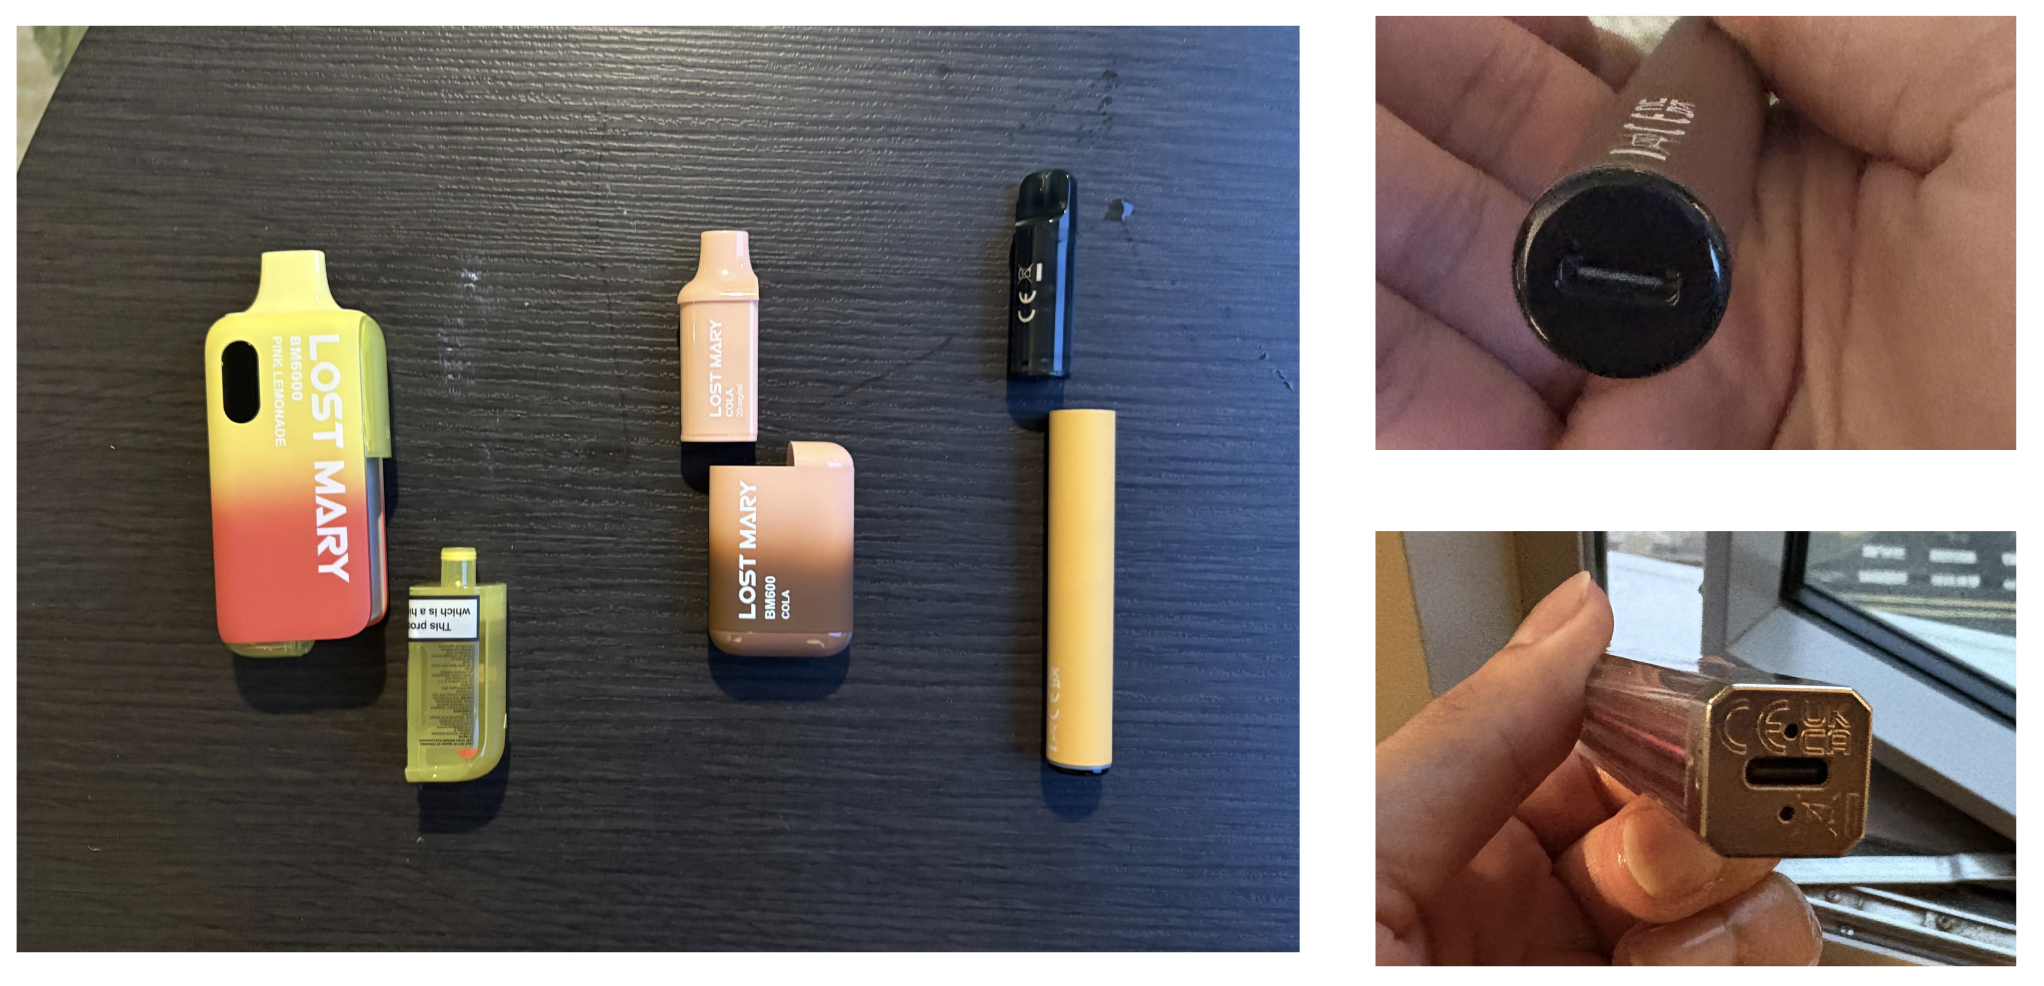
\includegraphics[width=0.7\linewidth]{vape aspects.png}
    \caption{Hardware adaptations to bypass legislation: USB charging ports and detachable pods added to low-capacity vapes.}
    \label{fig:vape_aspects}
\end{figure}

An unintended consequence of these design workarounds is that vape brands have arguably increased their environmental footprint by introducing yet another form of micro-litter: the detachable pod. Furthermore, during the procurement of the positive dataset inventory, retail vendors explicitly confirmed that they still view and sell these adapted devices as ``disposables.'' This reflects a systemic apathy toward recycling protocols. While poor disposal habits are common across many litter types, it is particularly severe in the context of vapes due to the formidable fire risk of the lithium-ion batteries and the toxicity of the chemical waste.

The physical unpackaging of the positive inventory (detailed in the Methodology) highlighted another critical issue: the excessive volume of ancillary, non-recyclable material included in vape packaging.

\begin{figure}[H]
    \centering
    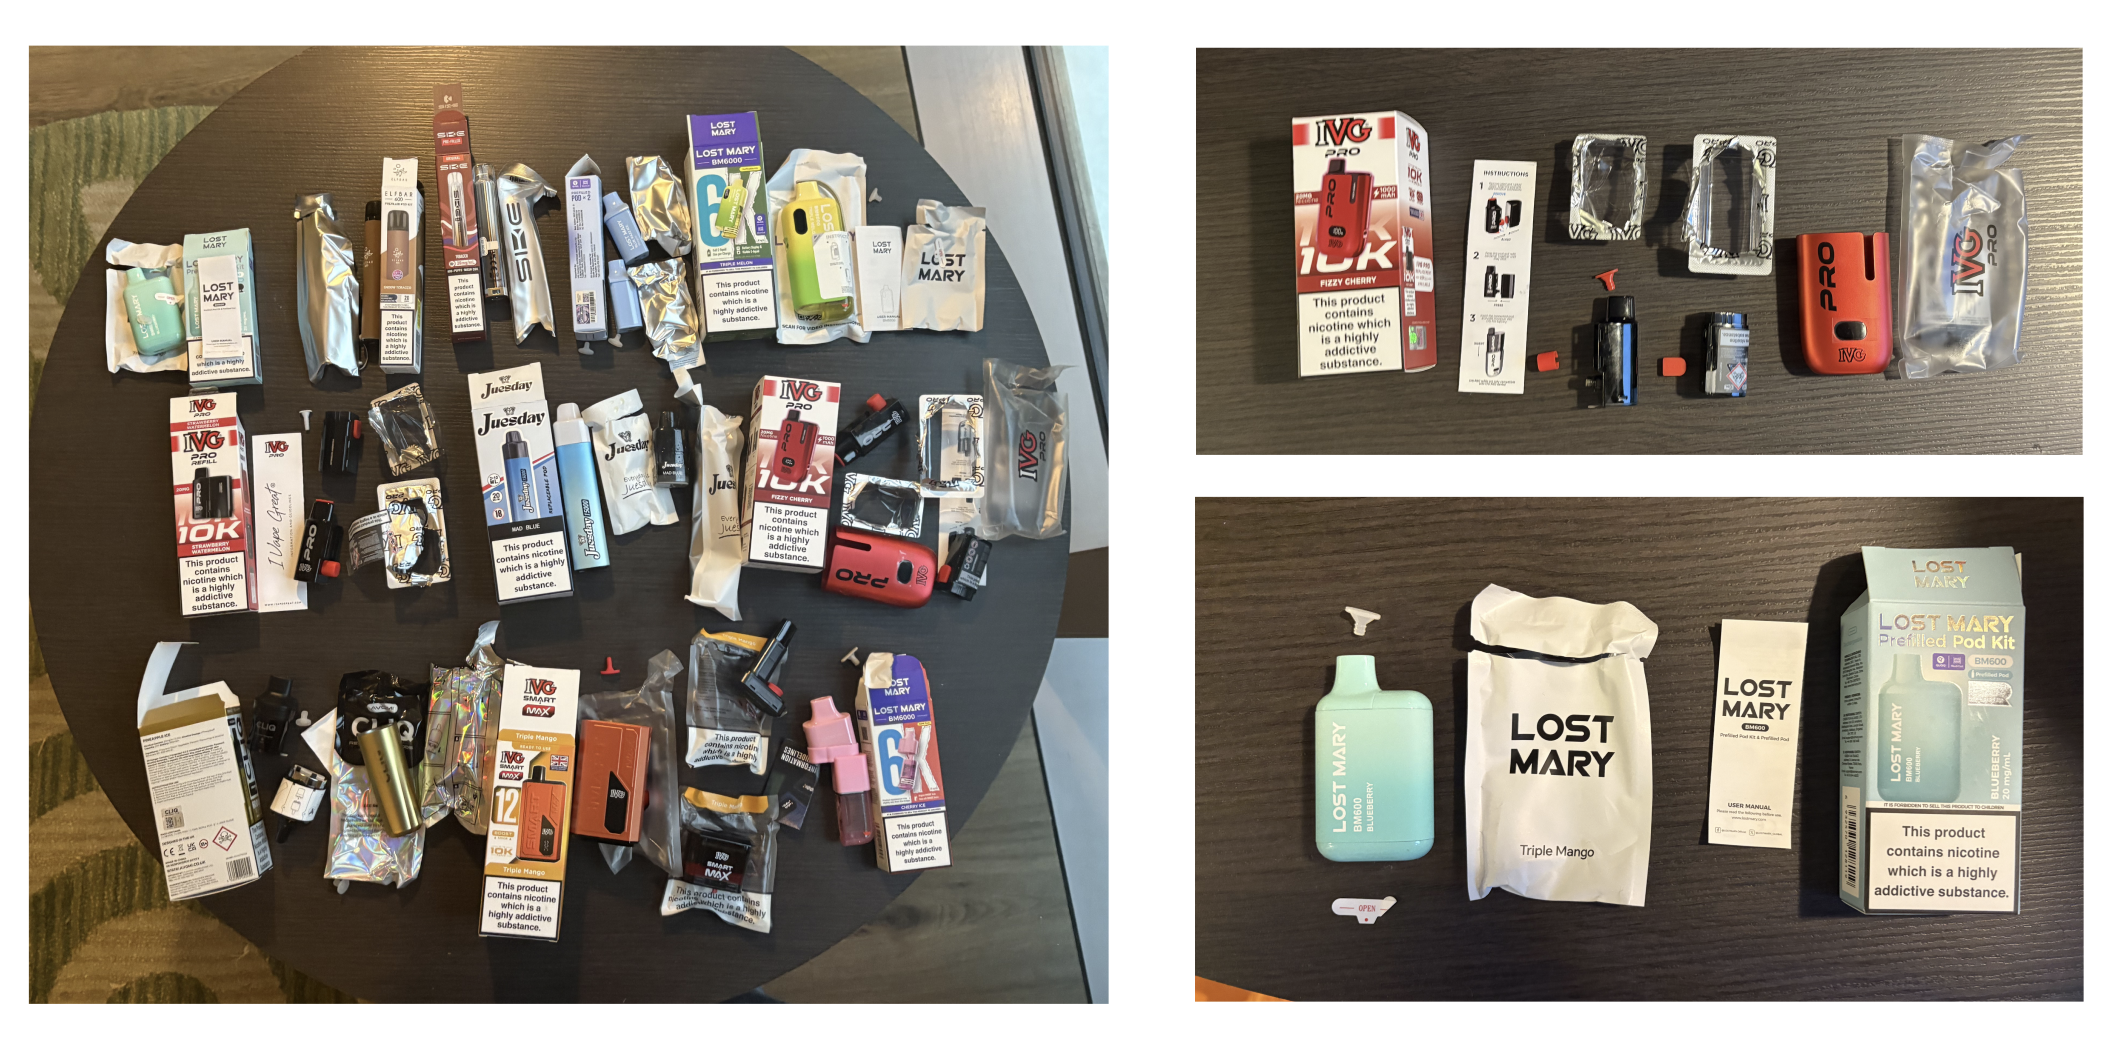
\includegraphics[width=0.7\linewidth]{Unpackaging of vape inventory.png}
    \caption{Unpackaging of the vape inventory: isolating the core device from the extensive secondary packaging and rubber seals.}
    \label{fig:unpackaging}
\end{figure}

This observation required a deliberate definition of the project's scope. The core assumption of the proposed detection model is that it exclusively tracks the vape device itself—ignoring the pods, rubber mouthpiece seals, plastic wrappers, and instruction manuals. This boundary was set to strictly isolate the primary micro-WEEE hazard (the battery). However, it is important to acknowledge that the vape industry is responsible for generating massive quantities of this fragmented secondary packaging, which contributes heavily to the types of small-scale litter that are incredibly difficult for manual cleaners to capture.

Additionally, during the unpackaging process, several devices leaked toxic e-liquid. This spillage serves as a direct, practical demonstration of the chemical hazard these devices pose to local environments and wildlife when damaged or degraded outdoors.

\begin{figure}[H]
    \centering
    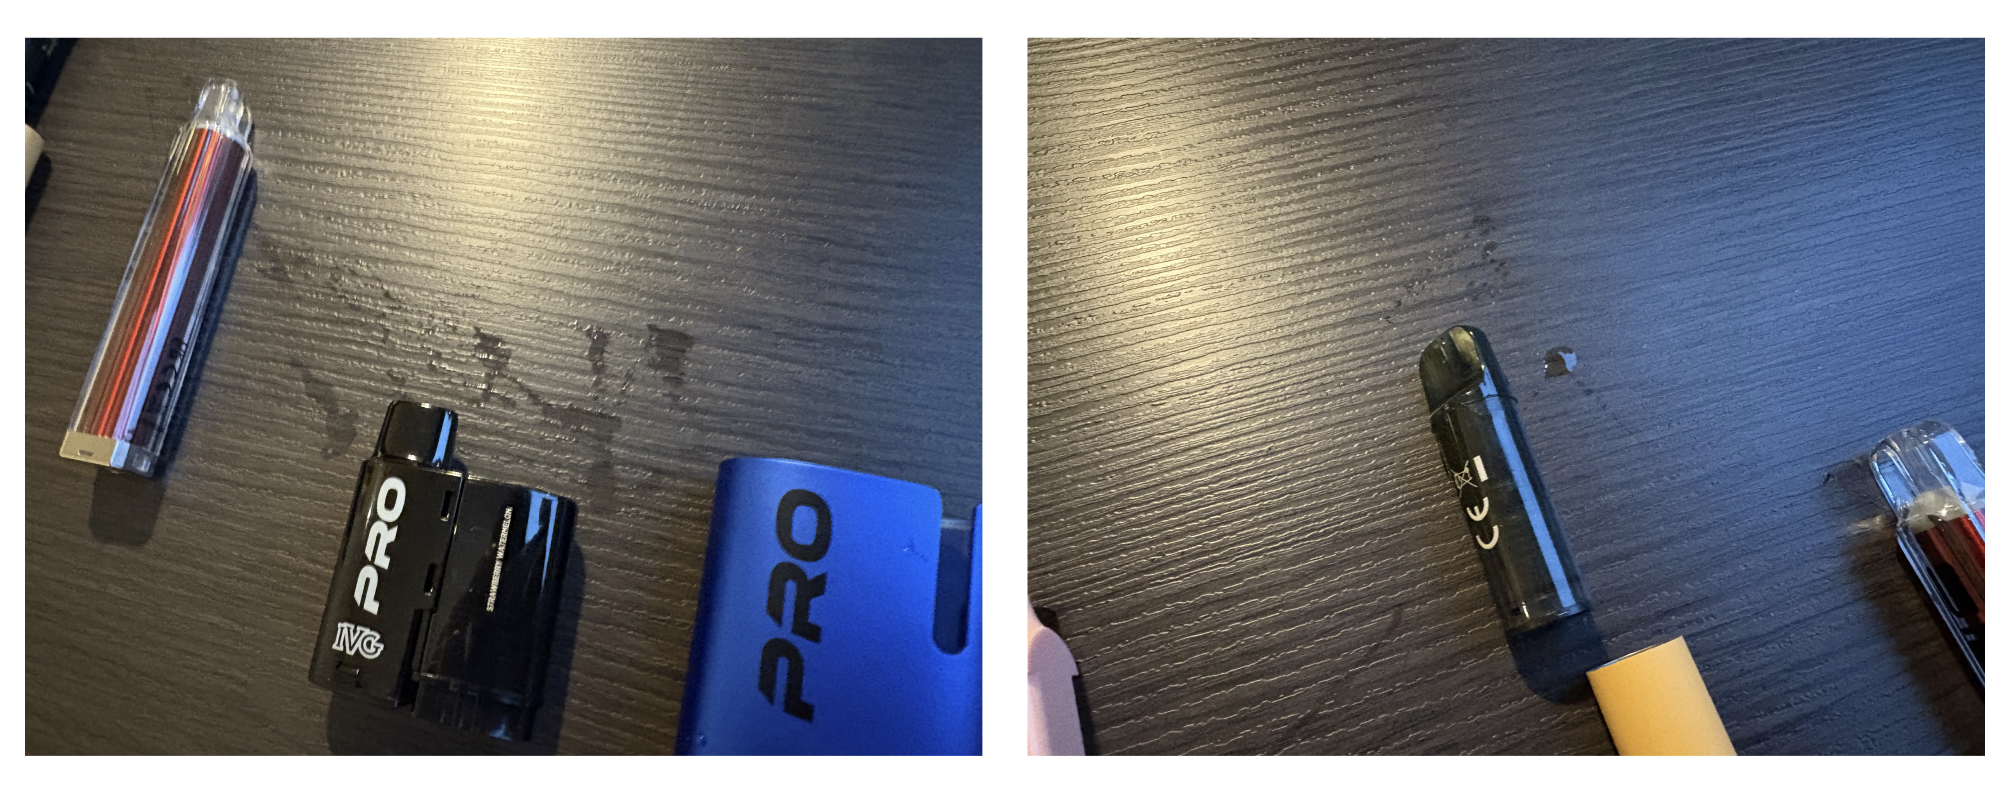
\includegraphics[width=0.7\linewidth]{Screenshot 2026-06-12 at 07.30.47.png}
    \caption{Toxic e-juice spillage occurring during the handling of new vape devices.}
    \label{fig:ejuice_spillage}
\end{figure}

The preparation of the dataset inventory generated a significant amount of this secondary waste. Care was taken by the researcher to sort and appropriately recycle all eligible packaging materials following the extraction of the target devices.

\begin{figure}[H]
    \centering
    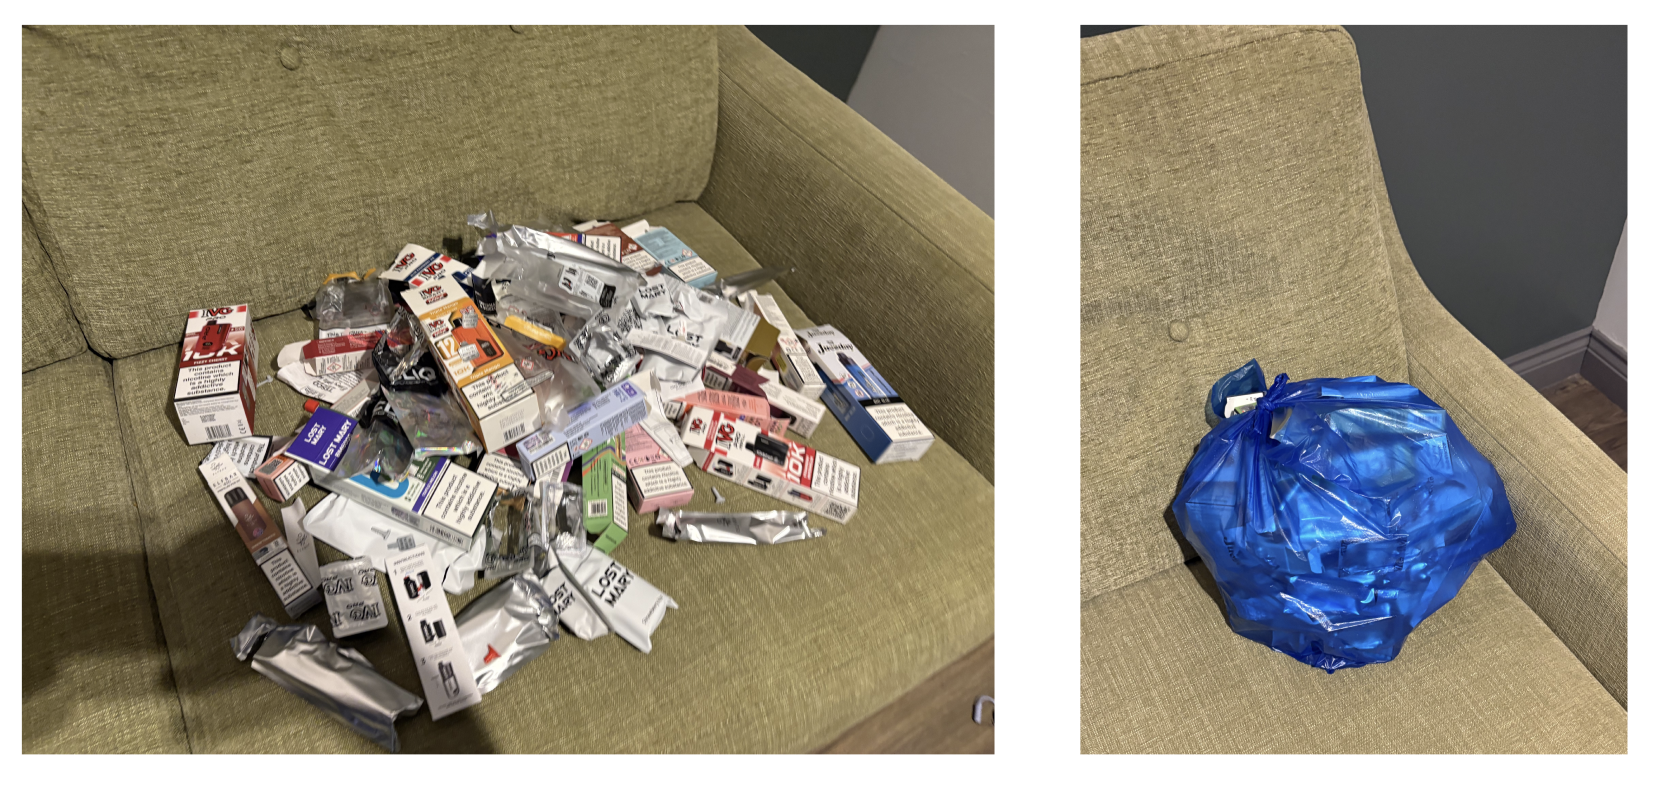
\includegraphics[width=0.7\linewidth]{Waste from unpackaging vape inventory.png}
    \caption{Consolidated secondary packaging waste generated from the positive inventory.}
    \label{fig:packaging_waste}
\end{figure}

\section{Further Investigation: Annotation Tools}
To contextualize the development of the Dataset Construction Engine (DCE), industry-standard annotation platforms were systematically evaluated. During this preliminary research phase, direct consultation with the CEO of DataTorch provided expert insight into the architectural design and structural challenges of scalable annotation systems. 

\begin{figure}[H]
    \centering
    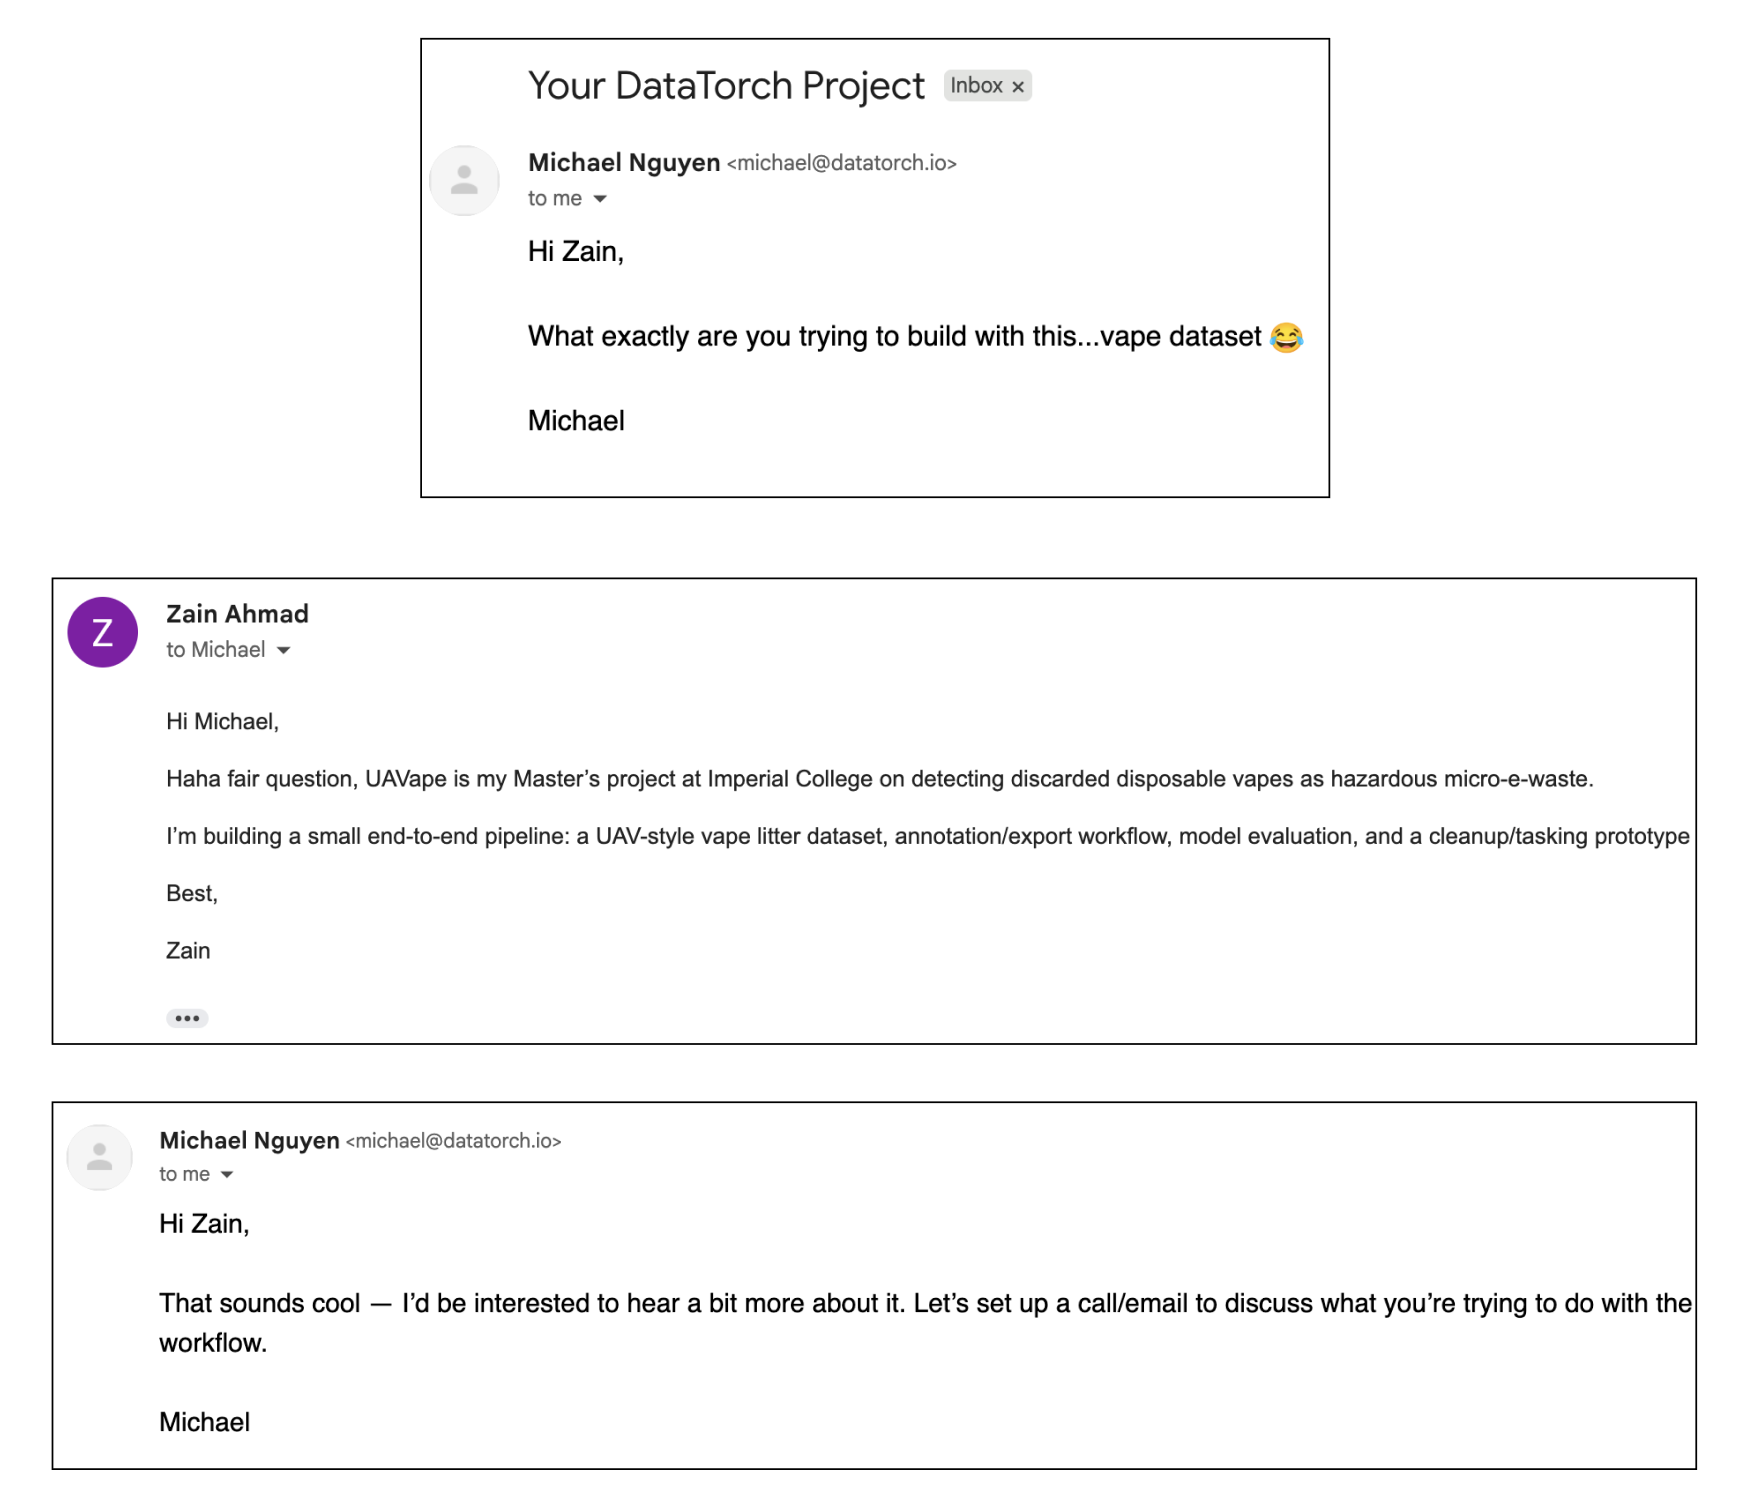
\includegraphics[width=0.7\linewidth]{emails.png}
    \caption{Initial expert correspondence with the CEO of DataTorch regarding annotation system architecture.}
    \label{fig:datatorch_email}
\end{figure}

While this correspondence yielded valuable operational context, DataTorch was ultimately excluded from the subsequent functional benchmark. It was a smaller annotation project compared with the remaining leading commercial platforms evaluated below.
% ==========================================
% APPENDIX TABLE BELOW
% ==========================================

\newcolumntype{Y}[1]{>{\raggedright\arraybackslash}p{#1}}

\begin{landscape}
\scriptsize
\setlength{\tabcolsep}{3pt}
\renewcommand{\arraystretch}{1.2}
\setlength{\LTleft}{0pt}
\setlength{\LTright}{0pt}

\begin{longtable}{@{}Y{0.10\linewidth}Y{0.15\linewidth}Y{0.15\linewidth}Y{0.15\linewidth}Y{0.15\linewidth}Y{0.15\linewidth}Y{0.15\linewidth}@{}}
\caption{Benchmark of industry-standard annotation tools against UAVape Dataset Construction Engine requirements.}
\label{tab:appendix_annotation_tool_benchmark}\\
\toprule
\textbf{Metric} &
\textbf{Metric Justification} &
\textbf{CVAT} &
\textbf{Label Studio} &
\textbf{Roboflow Annotate} &
\textbf{Ultralytics Platform} &
\textbf{V7 Darwin} \\
\midrule
\endfirsthead

\toprule
\textbf{Metric} &
\textbf{Metric Justification} &
\textbf{CVAT} &
\textbf{Label Studio} &
\textbf{Roboflow Annotate} &
\textbf{Ultralytics Platform} &
\textbf{V7 Darwin} \\
\midrule
\endhead

\midrule
\multicolumn{7}{r}{\textit{Continued on next page}}\\
\endfoot

\bottomrule
\endlastfoot

\textbf{Target user / audience} &
Clarifies whether the tool is designed for researchers, small teams, or full ML operations. &
Research and engineering teams needing open-source or self-hosted vision annotation. &
Flexible open-source labelling for many data types, including CV, NLP, and multimodal AI. &
Computer-vision developers wanting annotation, training, and deployment in one web workflow. &
YOLO-focused teams wanting to operate inside the Ultralytics ecosystem. &
Professional annotation teams needing image/video workflows and model-assisted labelling. \\

\textbf{Deployment / access model} &
Determines whether a tool fits lightweight research, self-hosted privacy, or paid enterprise deployment. &
Open-source self-hosted, cloud CVAT Online, and enterprise options. &
Open-source installable platform plus enterprise HumanSignal version. &
SaaS-first web platform with team workspaces and paid features. &
SaaS platform with cloud training and hosted deployment. &
Hosted Darwin platform with CLI, SDK, external storage, and workflow integrations. \\

\textbf{Annotation types} &
Measures whether the tool supports the visual labels needed for object detection and future segmentation. &
Boxes, polygons, masks, keypoints, skeletons, tracking, and 3D point-cloud tasks. &
Boxes, polygons, circular regions, keypoints, tracking, and semantic segmentation. &
Bounding boxes, polygons, masks, keypoints, and classification workflows. &
YOLO task coverage: detect boxes, segment polygons, pose keypoints, and oriented boxes. &
Bounding boxes, polygons, masks, brush tools, video, and specialist medical views. \\

\textbf{AI-assisted labelling} &
Crucial for small-object annotation to reduce labour via SAM-style assistance or model pre-labels. &
Supports automated annotation using pretrained/custom models; highlights SAM support. &
Supports ML backends and model pre-labelling, but requires complex project setup. &
Strong built-in AI: Label Assist, Smart Polygon/SAM, and Grounding-DINO-style Auto Label. &
Strong YOLO/SAM smart annotation, including own fine-tuned YOLO models. &
Strong Auto-Annotate, Auto-Track, SAM, and trained-model assisted labelling. \\

\textbf{Dataset fit \& Export} &
Captures whether labels can move cleanly into YOLO training and if versions are reproducible. &
Strong export support including YOLO, COCO, Pascal VOC, and 20+ formats. &
Strong API/SDK flexibility, but export depends heavily on project configuration. &
Very strong for CV datasets: manage, version, and download in YOLO training formats. &
Native YOLO dataset structure and numbered NDJSON snapshots for reproducible training. &
Strong imports/exports through Darwin CLI/SDK and documented CV export formats. \\

\textbf{Collaboration \& workflow} &
Indicates whether the tool can support task assignment and review rather than single-user drawing. &
Projects, tasks, jobs, roles, audit trails, progress tracking, and team workflows. &
Supports collaborative labelling, but workflow depth is locked behind enterprise deployments. &
Jobs, assignment, instructions, review mode, and approval/rejection. &
Team workflow exists, but is mainly tied to the YOLO model training lifecycle. &
Strong: workflow stages including annotate, review, consensus, archive, and sampling. \\

\textbf{Quality assurance / review} &
Essential for bounding-box quality, especially where tiny objects can be loosely labelled. &
Multi-stage validation, configurable thresholds, confusion matrix, and audit trails. &
Supports review and model-assisted correction, but QA process requires bespoke setup. &
Review mode with approve/reject, comments, label issues, and annotation insights. &
Useful class sidebar/counts, but less mature as a full QA workforce platform. &
Strong: review, consensus, workflow automation, and QA balance analytics. \\

\textbf{Fit for UAVape / small-object workflow} &
Evaluates suitability for high-resolution litter imagery, repeated QA, and export to detector training. &
High fit: open, self-hostable, robust CV annotation. May need custom UI for metadata. &
Medium-high fit: highly flexible, but less CV-specialised out of the box. &
High fit: fast web workflow and YOLO-friendly export. Less ideal if full DCE control is required. &
High fit for YOLO experiments; lower fit as a general-purpose annotation research environment. &
Medium-high fit: strong auto-annotation and review, but highly platform-dependent. \\

\textbf{Main limitation} &
Identifies why an off-the-shelf tool alone cannot satisfy the UAVape DCE requirements. &
Generic; scrape/synthetic provenance and bespoke metadata logic require heavy customisation. &
Configuration-heavy; not optimised solely for small-object CV out of the box. &
SaaS ``Walled Garden''; lacks native web-scraping and synthetic dataset bootstrapping tools. &
Narrow ecosystem focus; less suited to broad bespoke curation logic. &
Enterprise-first; strong annotation platform but lacks custom domain-specific creation flexibility. \\

\end{longtable}
\end{landscape}
\normalsize

\section{Further Investigation: Interviews with UK Cleaners}
\label{app:cleaner_interviews}
\textit{TODO: Insert Google Docs link for anonymised interview notes/transcripts, if permitted.}

This appendix item contains the supporting evidence for the cleaner investigation discussed in Section 3. The evidence should include the interview guide, anonymised notes or transcripts, and any coding notes used to identify the visibility, prioritisation and workflow themes.

\section{UAVape ML Method Iterations}
\label{appendix:uavape_ml_method_iterations}
\textit{TODO: Insert Google Docs link for the ML methods iteration logbook.}

This appendix item records the model-development process behind the final UAVape detector. It should include the benchmark runs, failed or discarded experiments, tiling branch, data-source ablations, final test command and any notes explaining why the final protocol was selected.

\section{UAVape Dataset}
\label{app:uavape_dataset_bundle}
\textit{TODO: Insert OneDrive link to the final UAVape dataset bundle.}

The dataset bundle should contain the three dataset sources used in this dissertation: the real UAVape detector dataset, the scraped vape-positive dataset and the synthetic vape-litter composite dataset. The real-image dataset should remain clearly separated from scraped and synthetic data because only real-world imagery was used for the sealed held-out test set.
\section{UAVape Detector Results Appendix}
\label{app:uavape_results_full_tables}

This appendix contains the full supporting tables for the UAVape detector-selection, tiling and data-source ablation results. The main results section extracts the same evidence and reports the more key findings.

\subsection{Full Aggregate Detector-Selection Ranking}

\begin{table}[H]
\centering
\scriptsize
\resizebox{\textwidth}{!}{%
\begin{tabular}{r l r r r r r}
\toprule
\textbf{Rank} & \textbf{Run} & \textbf{Best epoch} & \textbf{Precision} & \textbf{Recall} & \textbf{mAP50} & \textbf{mAP50--95} \\
\midrule
1 & YOLO26s @ 1280 & 77 & 0.83866 & 0.74882 & 0.80233 & 0.60501 \\
2 & YOLO11s @ 1280 & 74 & 0.83625 & 0.75079 & 0.78559 & 0.58851 \\
3 & YOLO11s @ 960 & 89 & 0.82587 & 0.74317 & 0.77487 & 0.56639 \\
4 & YOLO26m @ 640 & 82 & 0.77691 & 0.75584 & 0.79481 & 0.56215 \\
5 & YOLO26s @ 960 & 90 & 0.82190 & 0.68432 & 0.74253 & 0.54957 \\
6 & YOLO11n @ 960 & 90 & 0.84300 & 0.67100 & 0.76500 & 0.54500 \\
7 & YOLOv8s @ 1280 & 76 & 0.85542 & 0.66381 & 0.73735 & 0.54448 \\
8 & YOLO26s @ 640 & 71 & 0.82493 & 0.66468 & 0.76095 & 0.54024 \\
9 & YOLOv8s @ 960 & 89 & 0.82325 & 0.67099 & 0.73797 & 0.53573 \\
10 & YOLOv8m @ 640 & 88 & 0.78257 & 0.71402 & 0.75316 & 0.53368 \\
11 & YOLO26n @ 960 & 78 & 0.77300 & 0.68400 & 0.72900 & 0.52700 \\
12 & YOLO11m @ 640 & 81 & 0.86303 & 0.68856 & 0.75816 & 0.52415 \\
13 & YOLO11s @ 640 & 87 & 0.79727 & 0.69695 & 0.74736 & 0.50696 \\
14 & YOLOv8s @ 640 & 69 & 0.77860 & 0.68419 & 0.71935 & 0.48731 \\
15 & YOLO26n @ 640 & 74 & 0.74700 & 0.64300 & 0.68700 & 0.45900 \\
16 & YOLO11n @ 640 & 89 & 0.69900 & 0.68100 & 0.68800 & 0.45600 \\
\bottomrule
\end{tabular}}
\caption{Full aggregate validation ranking for the unified detector-selection benchmark.}
\label{tab:appendix_uavape_aggregate_validation}
\end{table}

\subsection{Full Vape-Class Detector-Selection Ranking}

\begin{table}[H]
\centering
\scriptsize
\resizebox{\textwidth}{!}{%
\begin{tabular}{r l r r r r}
\toprule
\textbf{Rank} & \textbf{Run} & \textbf{Vape precision} & \textbf{Vape recall} & \textbf{Vape AP50} & \textbf{Vape AP50--95} \\
\midrule
1 & YOLO26s @ 1280 & 0.90879 & 0.83851 & 0.91763 & 0.70669 \\
2 & YOLO26s @ 960 & 0.89150 & 0.77282 & 0.85692 & 0.68355 \\
3 & YOLO11s @ 1280 & 0.87633 & 0.84194 & 0.87978 & 0.67722 \\
4 & YOLO11s @ 960 & 0.88042 & 0.83833 & 0.90301 & 0.67675 \\
5 & YOLO26m @ 640 & 0.84197 & 0.84402 & 0.88876 & 0.66603 \\
6 & YOLOv8s @ 960 & 0.87992 & 0.80198 & 0.86633 & 0.65877 \\
7 & YOLOv8m @ 640 & 0.87599 & 0.80429 & 0.87318 & 0.64843 \\
8 & YOLO11m @ 640 & 0.87763 & 0.78218 & 0.88178 & 0.64840 \\
9 & YOLO26s @ 640 & 0.88375 & 0.73762 & 0.87651 & 0.64776 \\
10 & YOLO11n @ 960 & 0.87800 & 0.76200 & 0.87800 & 0.64500 \\
11 & YOLO11s @ 640 & 0.91750 & 0.79208 & 0.89317 & 0.63779 \\
12 & YOLO26n @ 960 & 0.82900 & 0.72800 & 0.83500 & 0.63300 \\
13 & YOLOv8s @ 1280 & 0.83696 & 0.73762 & 0.80318 & 0.61764 \\
14 & YOLO26n @ 640 & 0.84400 & 0.72800 & 0.82900 & 0.59800 \\
15 & YOLOv8s @ 640 & 0.85827 & 0.78218 & 0.83862 & 0.59569 \\
16 & YOLO11n @ 640 & 0.78000 & 0.80200 & 0.85300 & 0.58700 \\
\bottomrule
\end{tabular}}
\caption{Full vape-class validation ranking for the unified detector-selection benchmark.}
\label{tab:appendix_uavape_vape_validation}
\end{table}

\subsection{Nano Lower-Bound Results}

\begin{table}[H]
\centering
\scriptsize
\resizebox{\textwidth}{!}{%
\begin{tabular}{l r l l r r r r r r r r}
\toprule
\textbf{Run} & \textbf{Best epoch} & \textbf{Params / GFLOPs} & \textbf{Best weight size} & \textbf{Precision} & \textbf{Recall} & \textbf{mAP50} & \textbf{mAP50--95} & \textbf{Vape AP50} & \textbf{Vape AP50--95} & \textbf{Lighter AP50} & \textbf{Lighter AP50--95} \\
\midrule
YOLO26n @ 640 & 74 & 2.38M / 5.2 & 5.4 MB & 0.747 & 0.643 & 0.687 & 0.459 & 0.829 & 0.598 & 0.545 & 0.320 \\
YOLO26n @ 960 & 78 & 2.38M / 5.2 & 5.4 MB & 0.773 & 0.684 & 0.729 & 0.527 & 0.835 & 0.633 & 0.623 & 0.422 \\
YOLO11n @ 640 & 89 & 2.58M / 6.3 & 5.5 MB & 0.699 & 0.681 & 0.688 & 0.456 & 0.853 & 0.587 & 0.522 & 0.325 \\
YOLO11n @ 960 & 90 & 2.58M / 6.3 & 5.5 MB & 0.843 & 0.671 & 0.765 & 0.545 & 0.878 & 0.645 & 0.653 & 0.445 \\
\bottomrule
\end{tabular}}
\caption{Nano lower-bound validation results.}
\label{tab:appendix_uavape_nano}
\end{table}

\subsection{Lighter-Class Diagnostics}

\begin{table}[H]
\centering
\small
\begin{tabularx}{\textwidth}{l r r X}
\toprule
\textbf{Run} & \textbf{Lighter AP50} & \textbf{Lighter AP50--95} & \textbf{Interpretation} \\
\midrule
YOLO11s @ 1280 & 0.69071 & 0.50832 & Strongest lighter validation localisation result. \\
YOLO26s @ 1280 & 0.68792 & 0.49768 & Selected protocol; strongest vape result and close lighter diagnostic performance. \\
YOLO26m @ 640 & 0.70601 & 0.45521 & Strong lighter AP50, but weaker strict localisation than 1280 small models. \\
YOLO11n @ 960 & 0.65300 & 0.44500 & Best nano lighter diagnostic result. \\
\bottomrule
\end{tabularx}
\caption{Selected lighter-class validation diagnostics.}
\label{tab:appendix_uavape_lighter_diagnostic}
\end{table}

\subsection{Full SAHI Tiling Validation Branch}

\begin{table}[H]
\centering
\scriptsize
\resizebox{\textwidth}{!}{%
\begin{tabular}{l r r r r r r r}
\toprule
\textbf{Run} & \textbf{Predictions} & \textbf{All AP50} & \textbf{All AP50--95} & \textbf{Vape AP50} & \textbf{Vape AP50--95} & \textbf{Lighter AP50} & \textbf{Lighter AP50--95} \\
\midrule
YOLO26s @ 640 + SAHI 1280/20\% & 9131 & 0.63982 & 0.48436 & 0.72741 & 0.55774 & 0.55223 & 0.41098 \\
YOLO26s @ 960 + SAHI 1280/20\% & 7568 & 0.69592 & 0.51027 & 0.80554 & 0.60559 & 0.58631 & 0.41494 \\
YOLO11s @ 960 + SAHI 1280/20\% & 10449 & 0.68078 & 0.51124 & 0.76595 & 0.58479 & 0.59561 & 0.43769 \\
YOLO11n @ 960 + SAHI 1280/20\% & 14250 & 0.67804 & 0.50773 & 0.75871 & 0.56937 & 0.59736 & 0.44609 \\
\bottomrule
\end{tabular}}
\caption{Full SAHI-style tiled inference validation results.}
\label{tab:appendix_uavape_sahi}
\end{table}

\subsection{Data-Source Ablation Recipes}

\begin{table}[H]
\centering
\scriptsize
\resizebox{\textwidth}{!}{%
\begin{tabular}{l l r r r r}
\toprule
\textbf{Run} & \textbf{Training recipe} & \textbf{Train images} & \textbf{Train boxes} & \textbf{Vape boxes} & \textbf{Lighter boxes} \\
\midrule
\texttt{A0\_real\_only} & V4 real train only & 837 & 1317 & 870 & 447 \\
\texttt{S88\_scraped} & V4 real + 88 scraped vape images & 925 & 1440 & 993 & 447 \\
\texttt{S177\_scraped} & V4 real + 177 scraped vape images & 1014 & 1579 & 1132 & 447 \\
\texttt{S355\_scraped} & V4 real + 355 scraped vape images & 1192 & 1864 & 1417 & 447 \\
\texttt{Y88\_synthetic} & V4 real + 88 synthetic vape images & 925 & 1405 & 958 & 447 \\
\texttt{Y177\_synthetic} & V4 real + 177 synthetic vape images & 1014 & 1494 & 1047 & 447 \\
\texttt{Y355\_synthetic} & V4 real + 355 synthetic vape images & 1192 & 1672 & 1225 & 447 \\
\texttt{S355\_Y355\_combined} & V4 real + 355 scraped + 355 synthetic vape images & 1547 & 2219 & 1772 & 447 \\
\bottomrule
\end{tabular}}
\caption{Training recipes used in the V4 data-source ablation.}
\label{tab:appendix_uavape_ablation_recipes}
\end{table}

\subsection{Full Data-Source Ablation Validation Results}

\begin{table}[H]
\centering
\scriptsize
\resizebox{\textwidth}{!}{%
\begin{tabular}{l r r r r r r r r r r r r}
\toprule
\textbf{Run} & \textbf{All P} & \textbf{All R} & \textbf{All AP50} & \textbf{All AP50--95} & \textbf{Vape P} & \textbf{Vape R} & \textbf{Vape AP50} & \textbf{Vape AP50--95} & \textbf{Lighter P} & \textbf{Lighter R} & \textbf{Lighter AP50} & \textbf{Lighter AP50--95} \\
\midrule
\texttt{A0\_real\_only} & 0.839 & 0.749 & 0.802 & 0.605 & 0.909 & 0.839 & 0.918 & 0.707 & 0.770 & 0.660 & 0.688 & 0.498 \\
\texttt{S88\_scraped} & 0.860 & 0.739 & 0.774 & 0.601 & 0.907 & 0.797 & 0.874 & 0.696 & 0.812 & 0.680 & 0.675 & 0.506 \\
\texttt{S177\_scraped} & 0.861 & 0.746 & 0.799 & 0.619 & 0.897 & 0.821 & 0.899 & 0.720 & 0.825 & 0.670 & 0.699 & 0.519 \\
\texttt{S355\_scraped} & 0.833 & 0.709 & 0.777 & 0.611 & 0.910 & 0.797 & 0.891 & 0.718 & 0.756 & 0.621 & 0.663 & 0.505 \\
\texttt{Y88\_synthetic} & 0.874 & 0.721 & 0.803 & 0.617 & 0.925 & 0.792 & 0.912 & 0.712 & 0.823 & 0.649 & 0.694 & 0.522 \\
\texttt{Y177\_synthetic} & 0.867 & 0.716 & 0.792 & 0.598 & 0.897 & 0.822 & 0.903 & 0.692 & 0.838 & 0.610 & 0.681 & 0.504 \\
\texttt{Y355\_synthetic} & 0.797 & 0.747 & 0.793 & 0.616 & 0.888 & 0.824 & 0.898 & 0.716 & 0.706 & 0.670 & 0.687 & 0.516 \\
\texttt{S355\_Y355\_combined} & 0.833 & 0.774 & 0.815 & 0.639 & 0.905 & 0.853 & 0.922 & 0.737 & 0.760 & 0.695 & 0.708 & 0.541 \\
\bottomrule
\end{tabular}}
\caption{Full validation results from the V4 data-source ablation.}
\label{tab:appendix_uavape_ablation_full_validation}
\end{table}

\subsection{Supporting Graphical Evidence}

This appendix section provides supporting graphical outputs from the UAVape detector experiments. These figures complement the quantitative results by showing training behaviour, class-level confusion, precision--recall behaviour and representative prediction outputs for the selected model runs.

\subsubsection{Detector-Selection Run}

\begin{figure}[H]
    \centering
    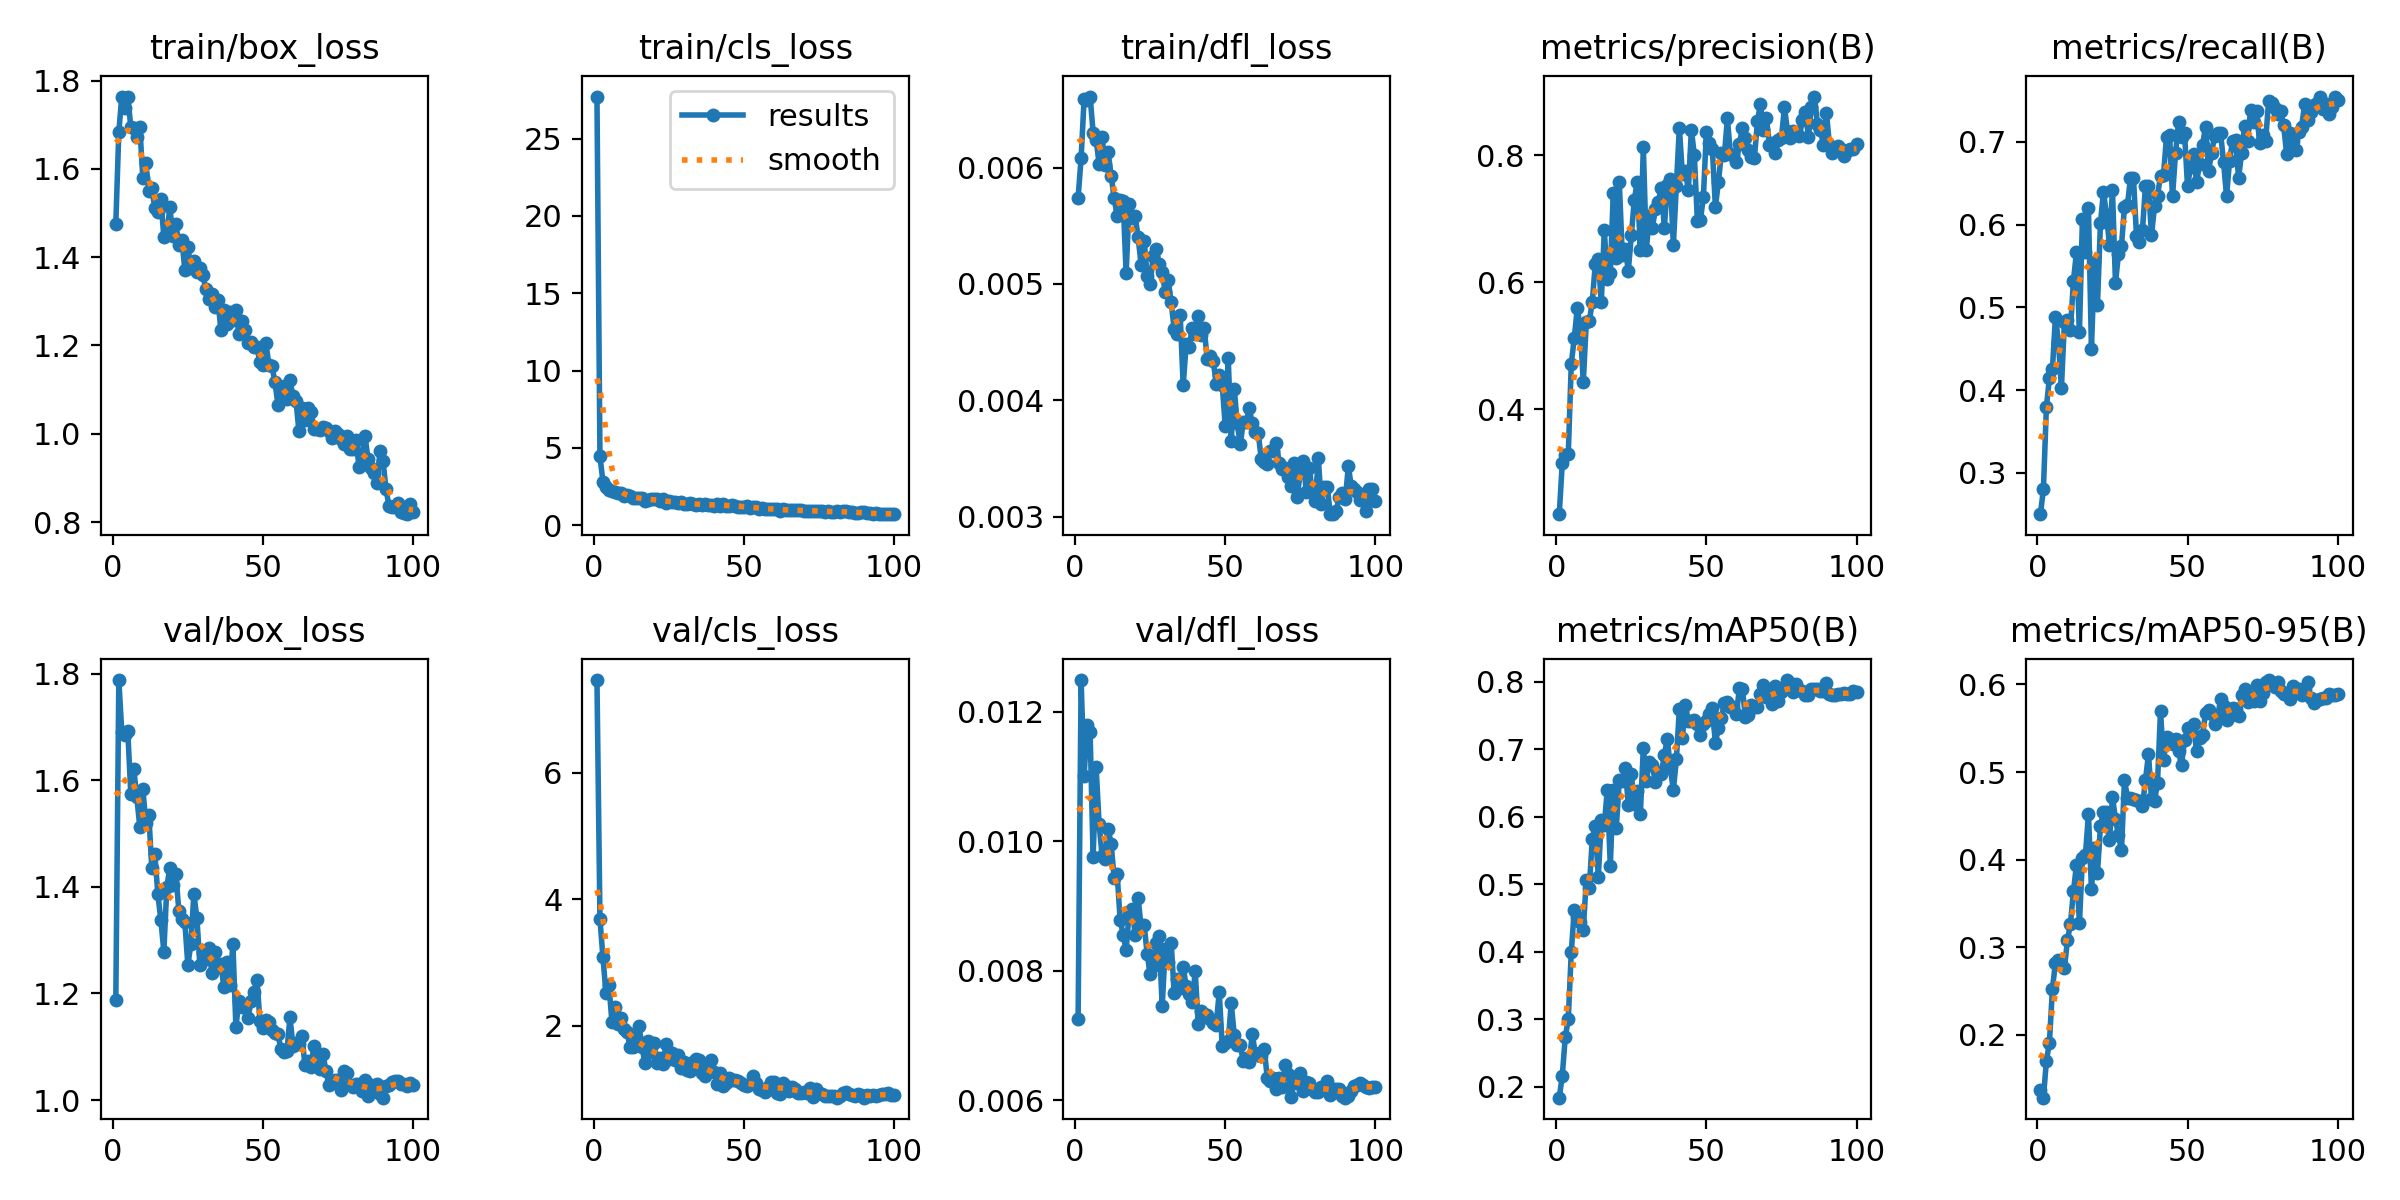
\includegraphics[width=0.85\linewidth]{yolo26s_img1280_training_curves.png}
    \caption{Training and validation curves for the selected detector-selection run, \texttt{YOLO26s@1280}. The curves provide the training trace for the validation-selected model before the later data-source ablation stage.}
    \label{fig:appendix_yolo26s_1280_training_curves}
\end{figure}

\begin{figure}[H]
    \centering
    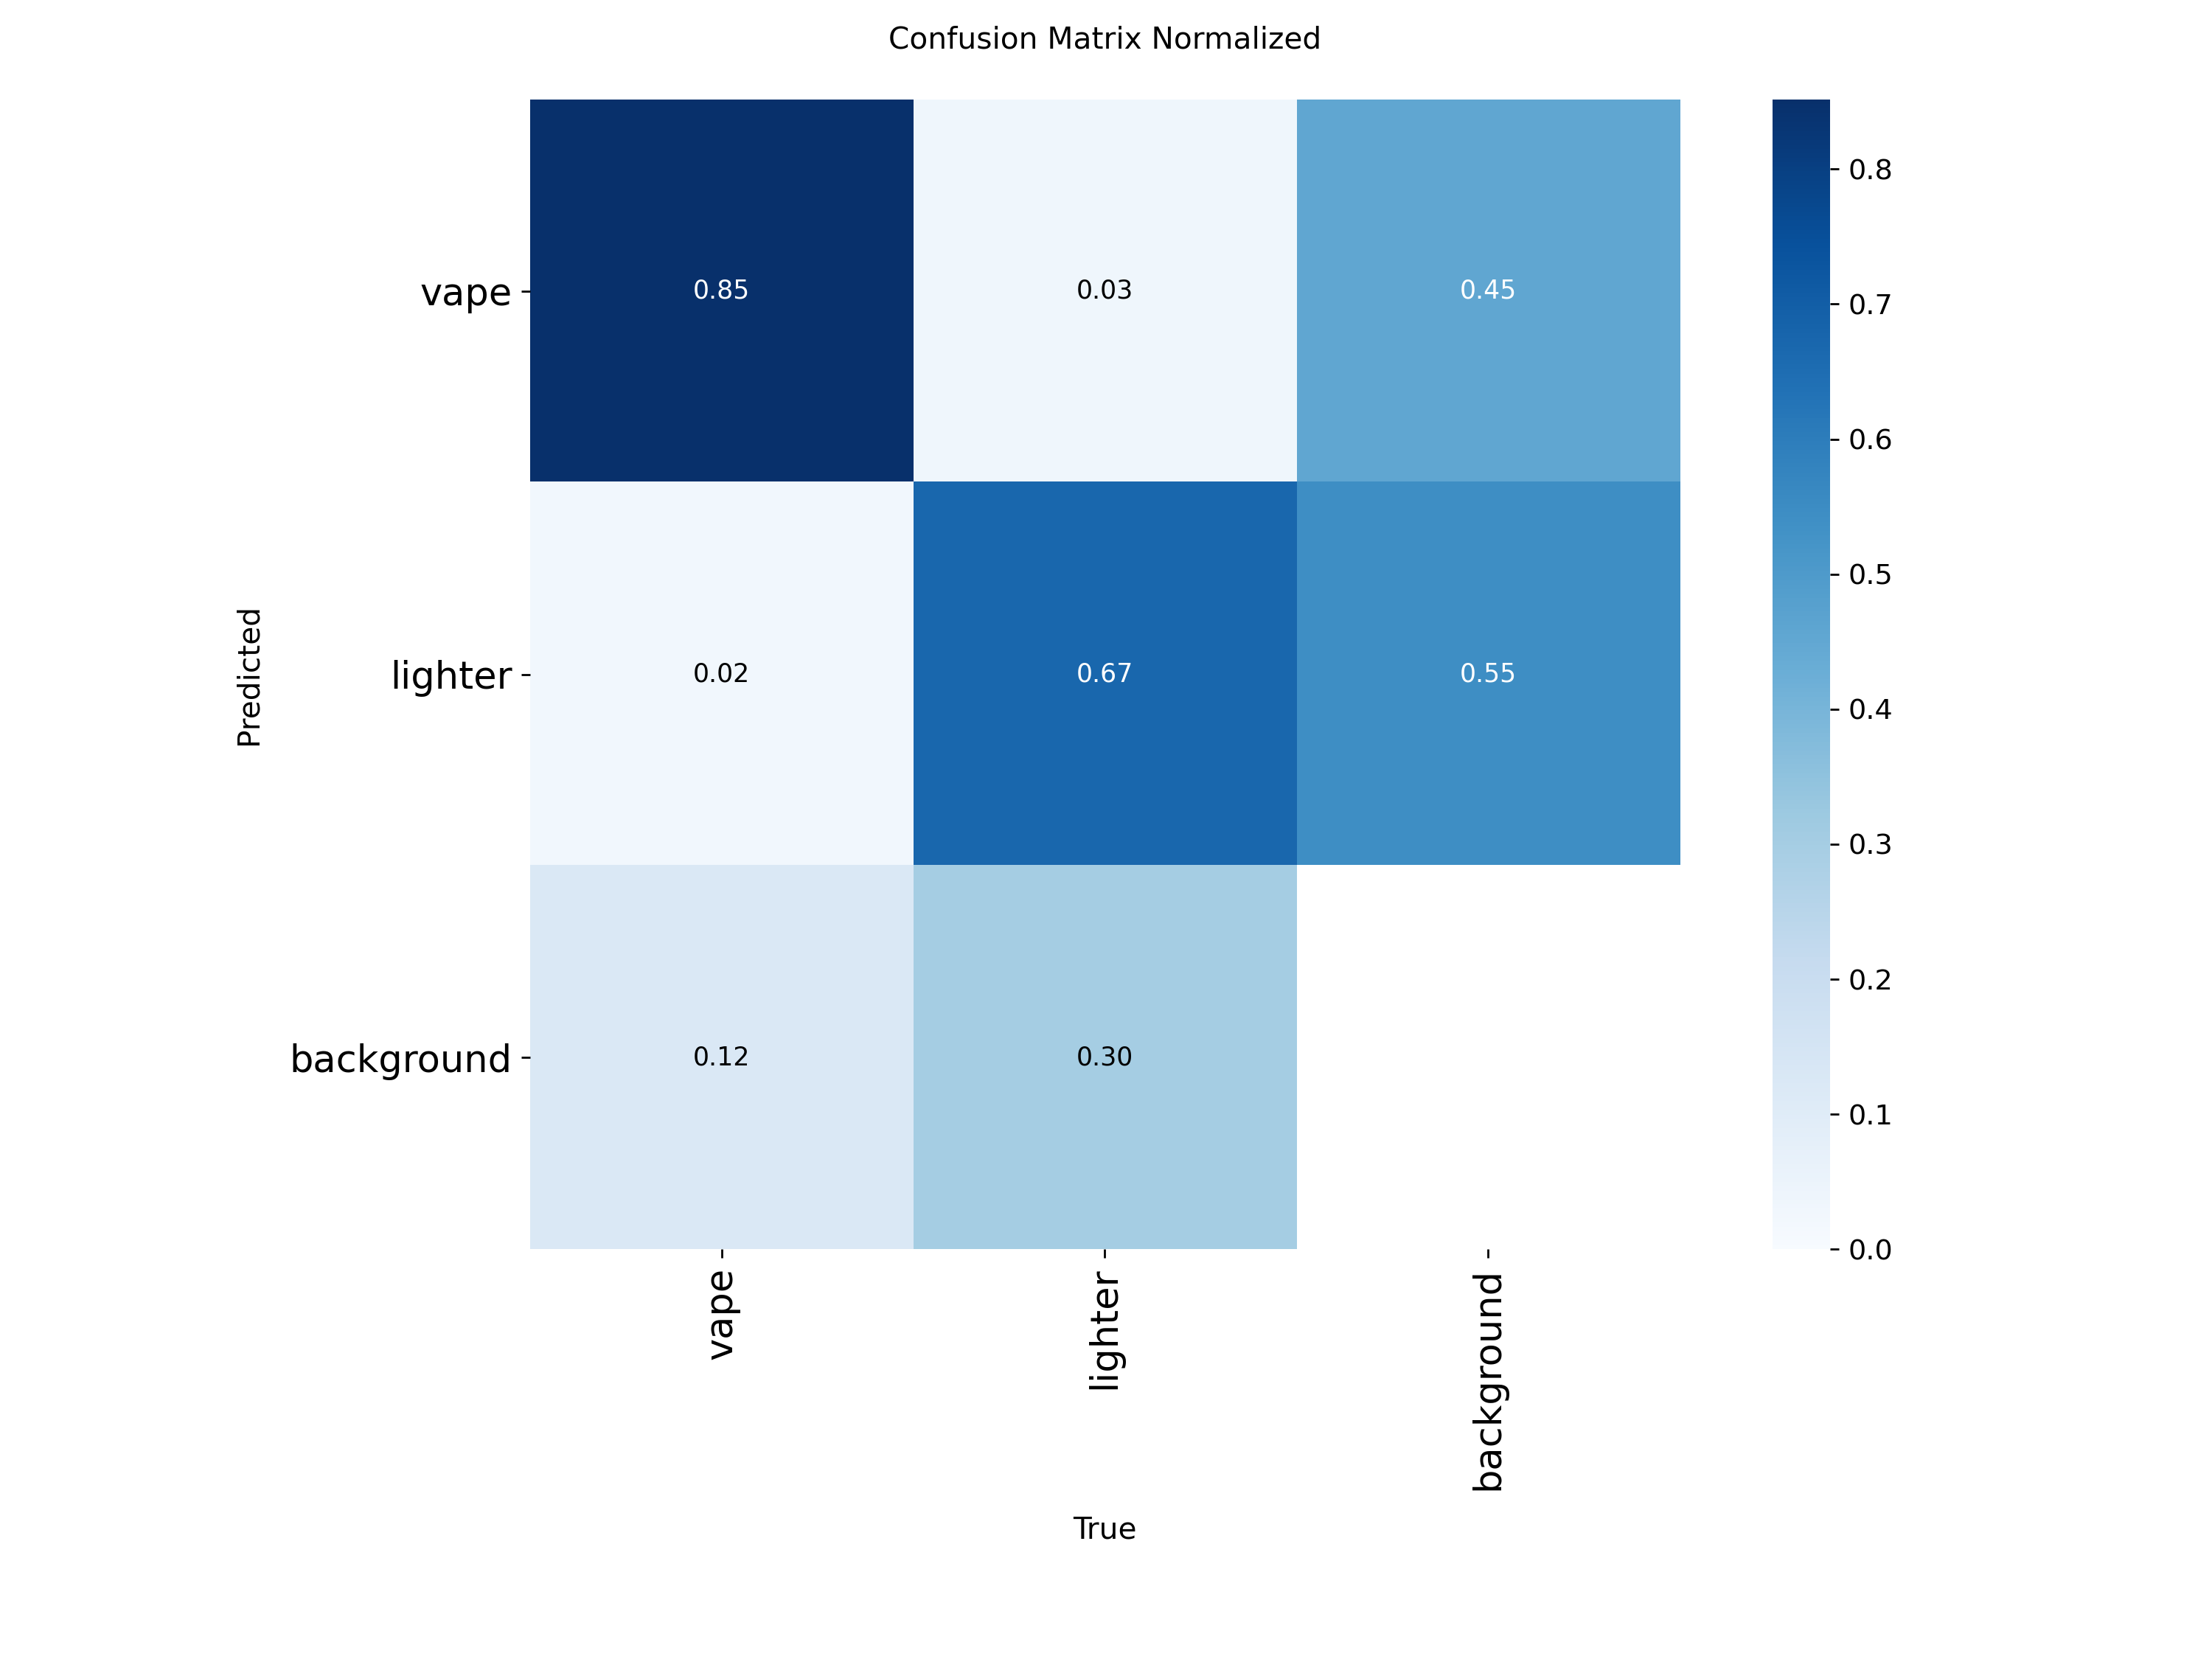
\includegraphics[width=0.62\linewidth]{yolo26s_img1280_confusion_matrix_normalized.png}
    \caption{Normalised validation confusion matrix for the selected \texttt{YOLO26s@1280} detector-selection run. This figure shows class-level behaviour for the initial real-data detector protocol, before adding scraped and synthetic source data.}
    \label{fig:appendix_yolo26s_1280_confusion_matrix}
\end{figure}

\subsubsection{Selected Data-Ablation Run}

\begin{figure}[H]
    \centering
    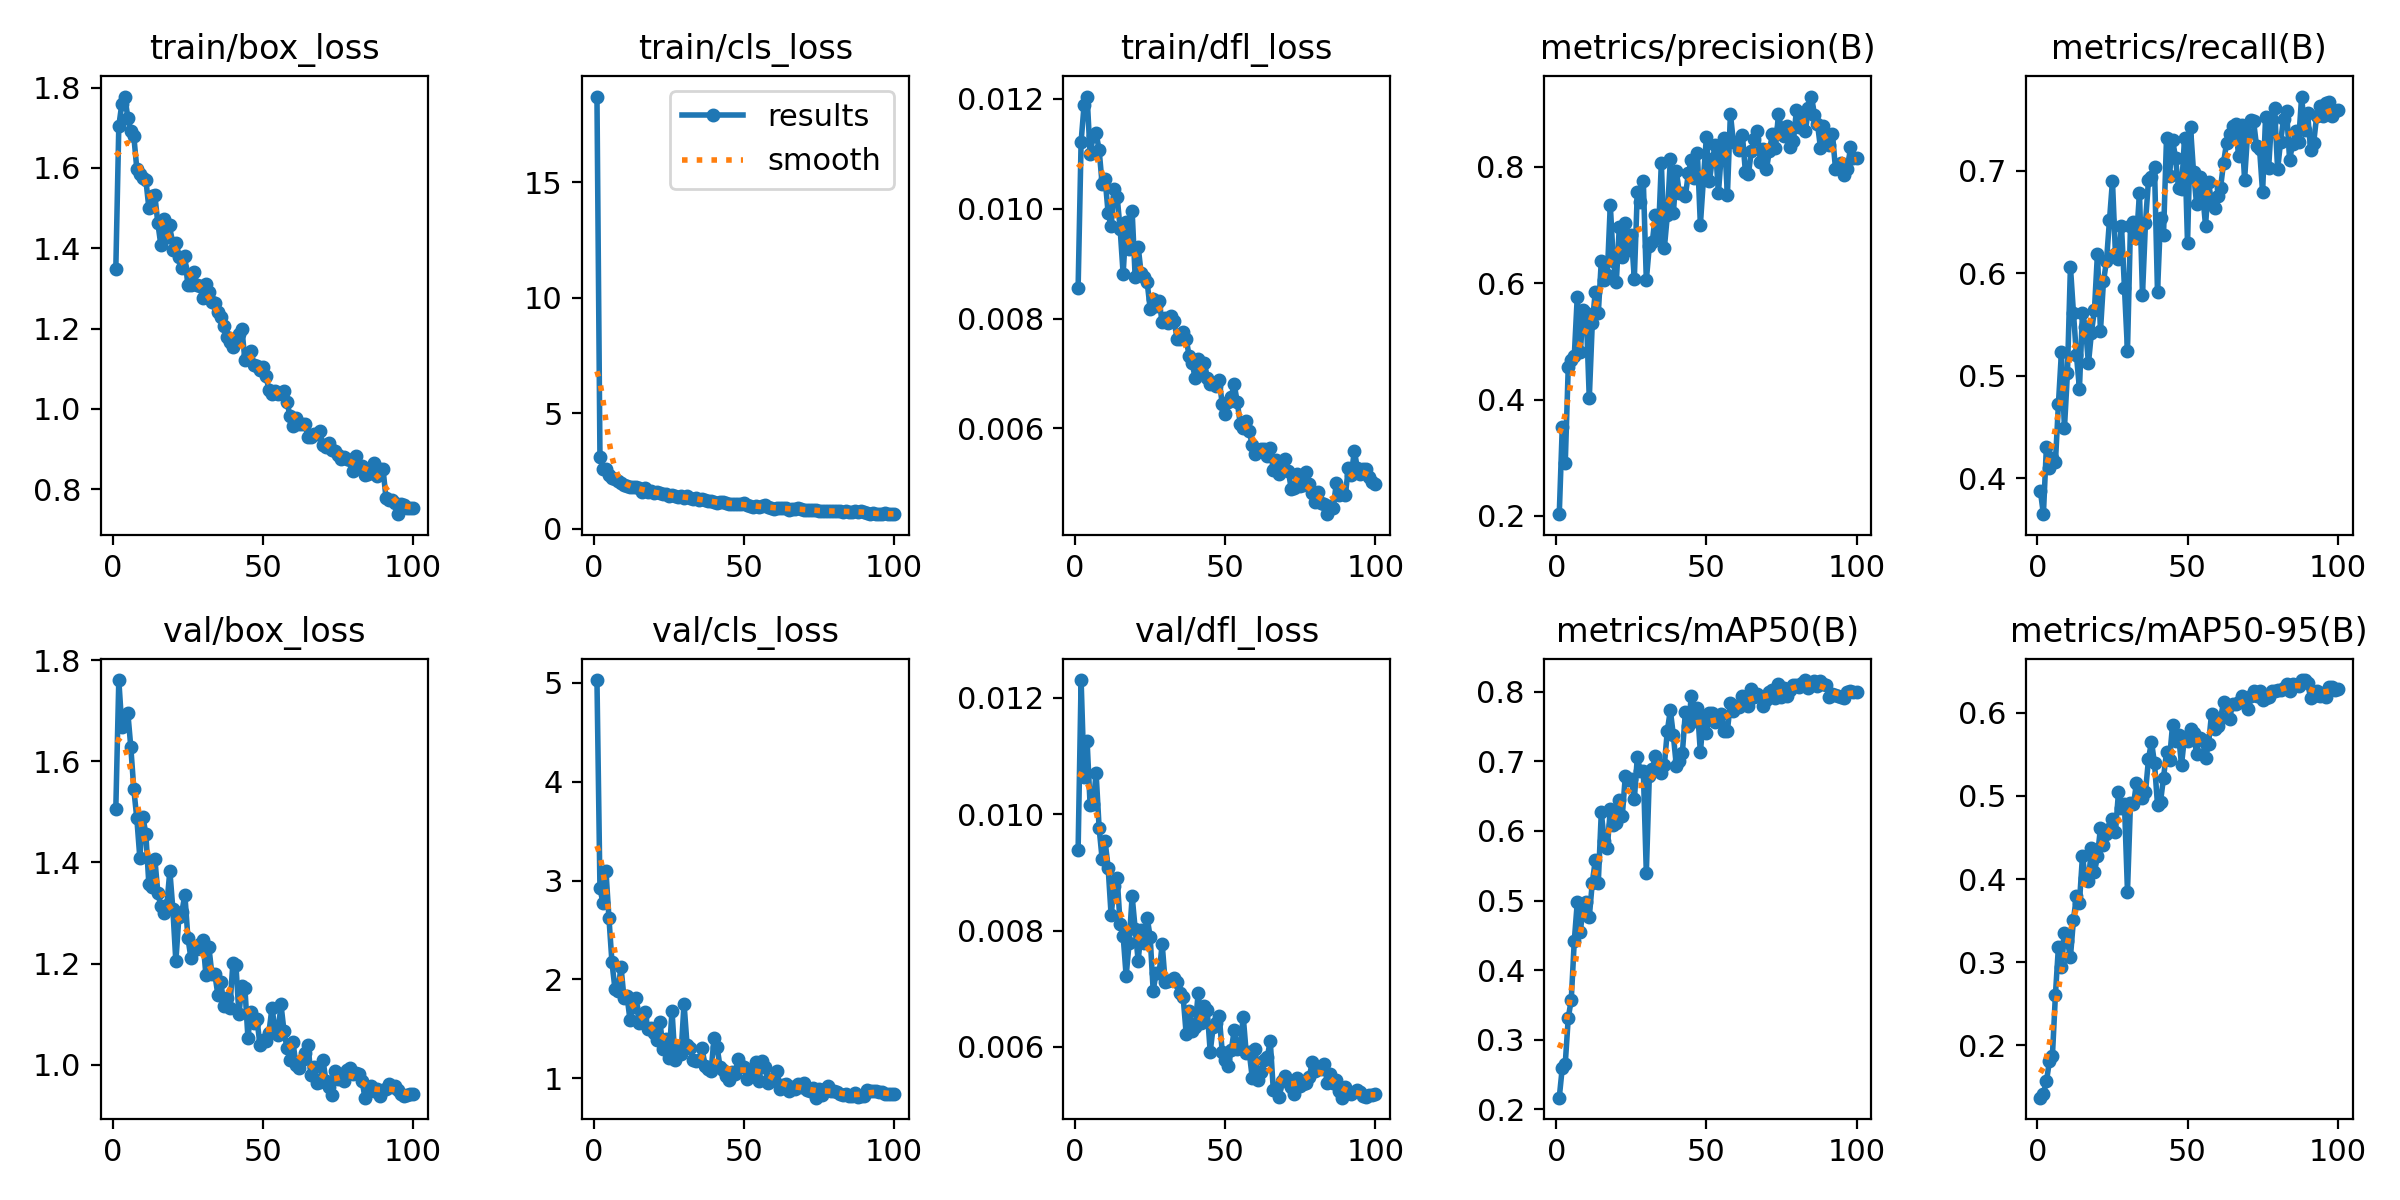
\includegraphics[width=0.85\linewidth]{s355_y355_combined_training_curves.png}
    \caption{Training and validation curves for the selected data-ablation run, \texttt{S355\_Y355\_combined}. This run used the fixed \texttt{YOLO26s@1280} protocol with the combined scraped-plus-synthetic training recipe.}
    \label{fig:appendix_s355_y355_training_curves}
\end{figure}

\begin{figure}[H]
    \centering
    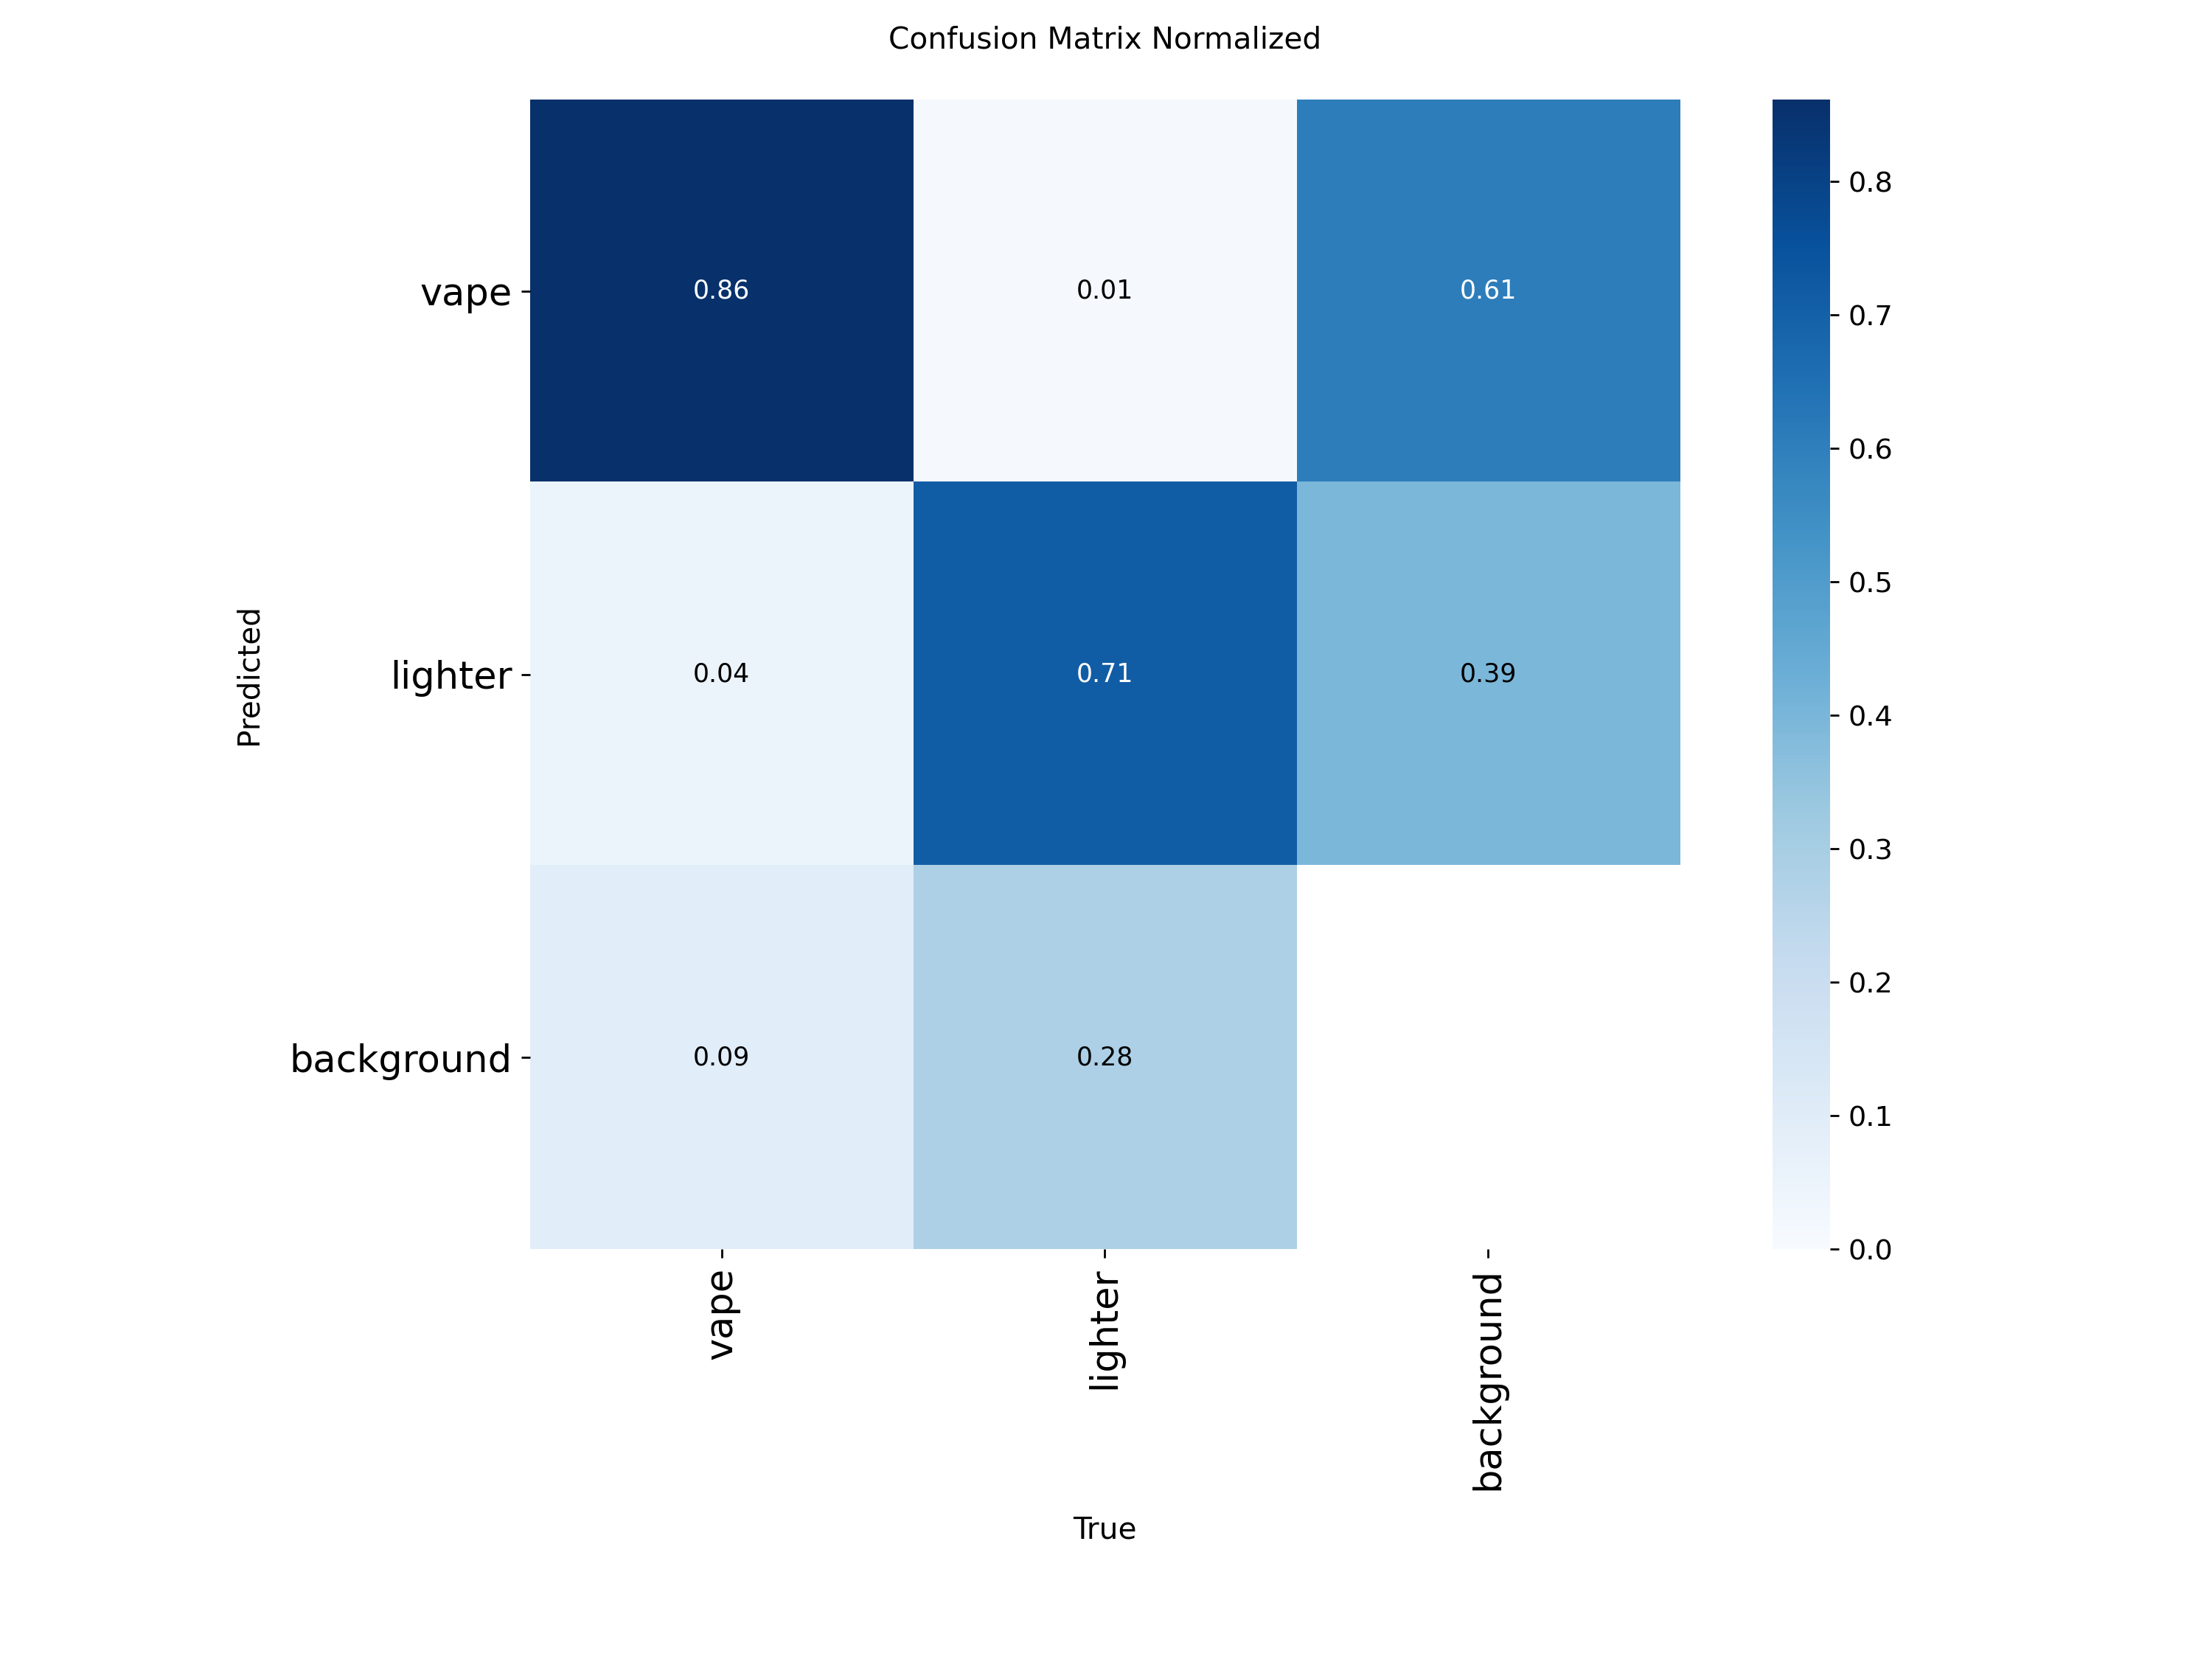
\includegraphics[width=0.62\linewidth]{s355_y355_combined_confusion_matrix_normalized.png}
    \caption{Normalised validation confusion matrix for the selected \texttt{S355\_Y355\_combined} data-ablation run. This figure supports the validation result used to select the final checkpoint for sealed test evaluation.}
    \label{fig:appendix_s355_y355_confusion_matrix}
\end{figure}

\subsubsection{Final Sealed-Test Evaluation}

\begin{figure}[H]
    \centering
    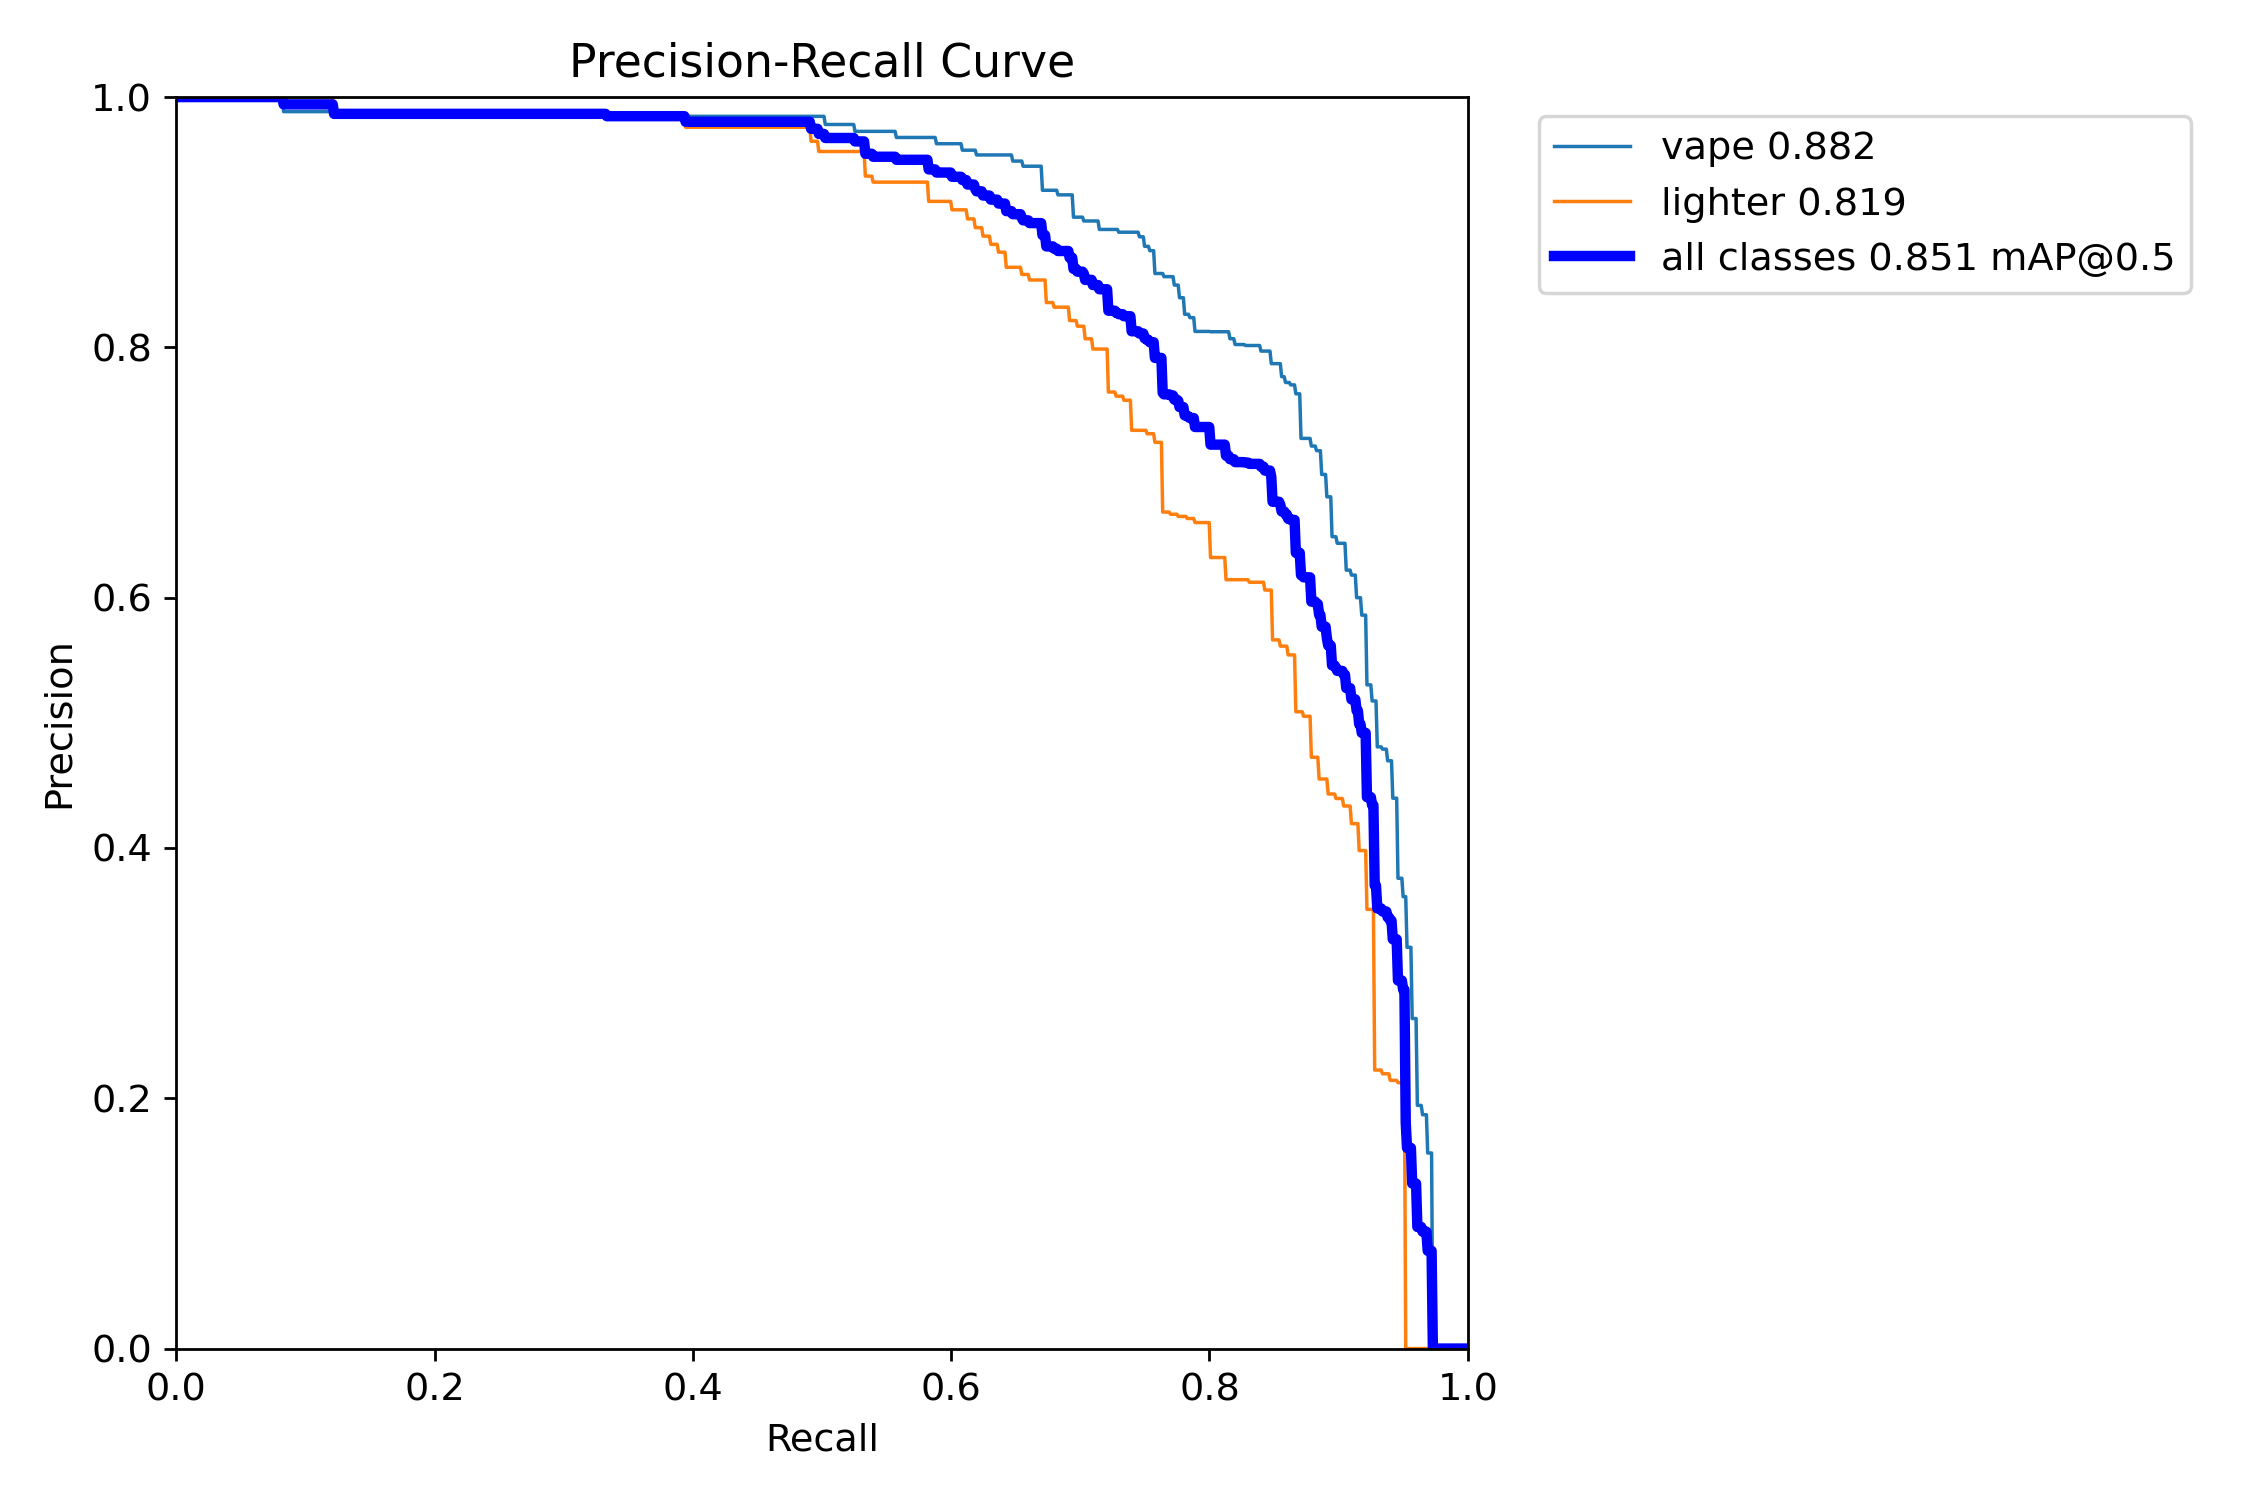
\includegraphics[width=0.70\linewidth]{final_test_PR_curve.png}
    \caption{Precision--recall curve for the final sealed-test evaluation of the selected \texttt{S355\_Y355\_combined} checkpoint. This figure visualises the target detector's confidence-threshold behaviour on the held-out test split.}
    \label{fig:appendix_final_test_pr_curve}
\end{figure}

\begin{figure}[H]
    \centering
    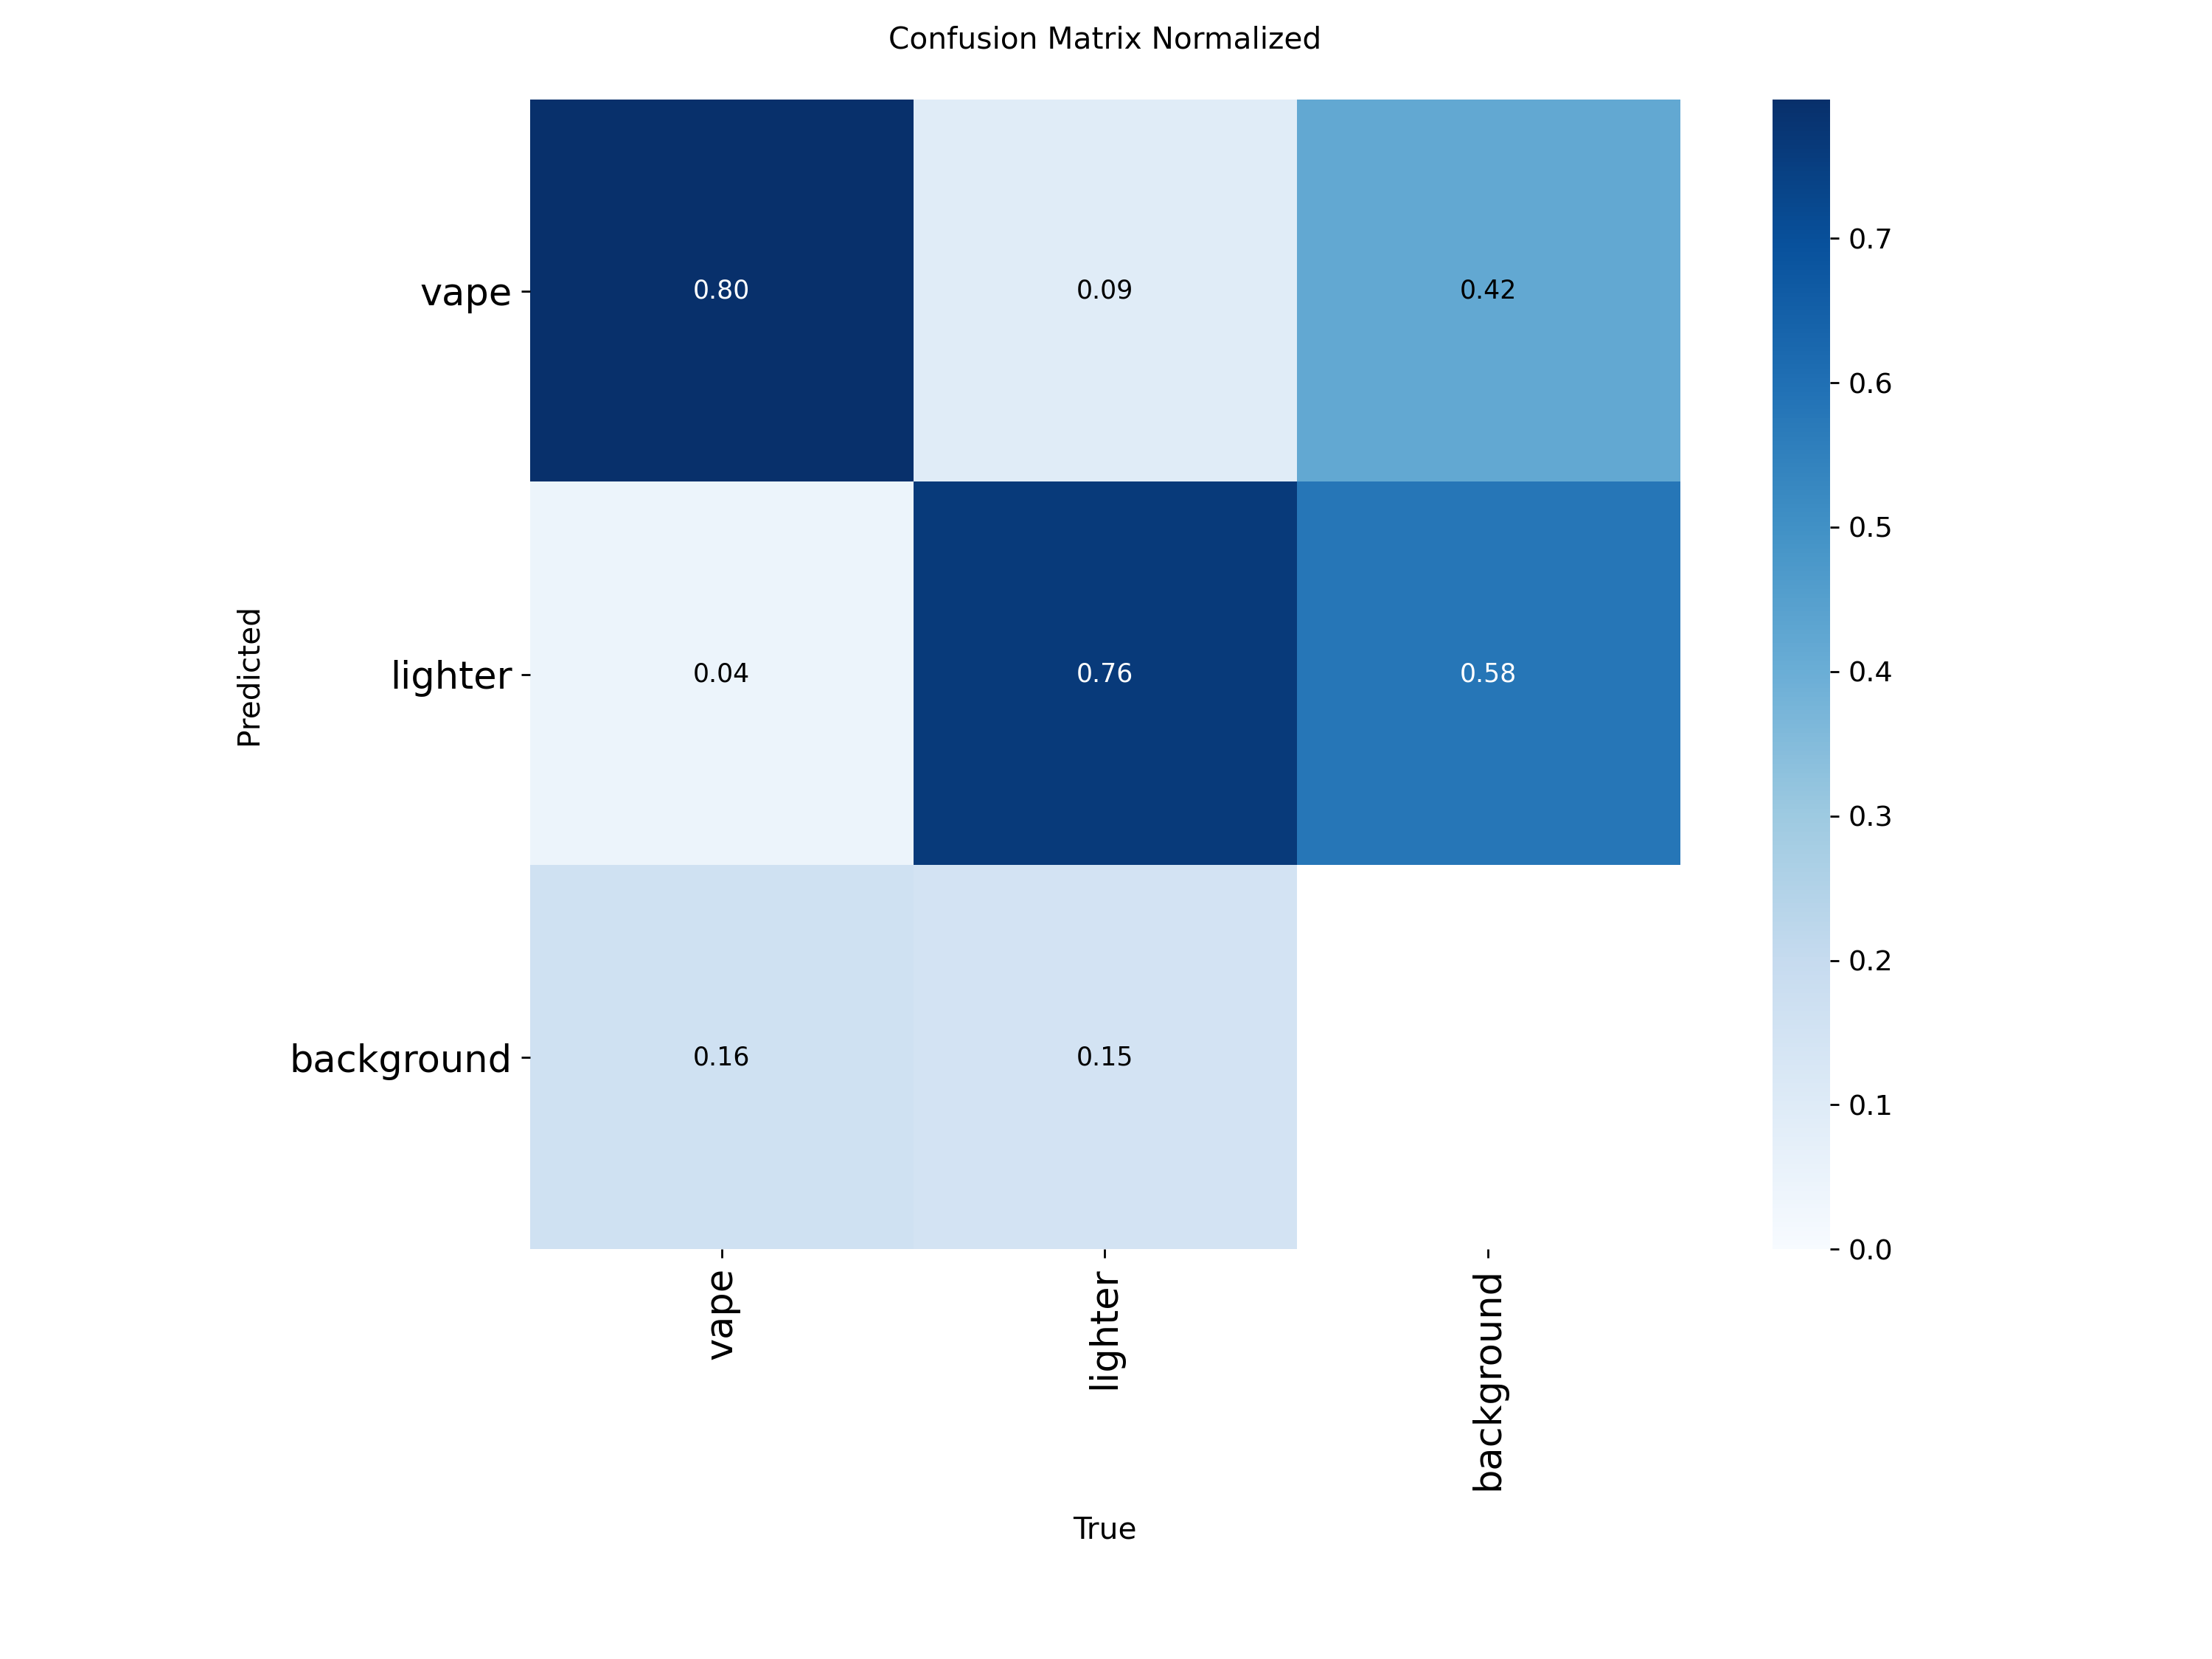
\includegraphics[width=0.62\linewidth]{final_test_confusion_matrix_normalized.png}
    \caption{Normalised confusion matrix for the final sealed-test evaluation. This figure provides class-level diagnostic evidence for the final reported test metrics.}
    \label{fig:appendix_final_test_confusion_matrix}
\end{figure}

\subsubsection{Final Prediction Previews}

The following prediction previews show representative final-test batches generated by the selected detector. They are included to provide qualitative context for the numerical test metrics, showing how detections appear on held-out real images.

\begin{figure}[H]
    \centering
    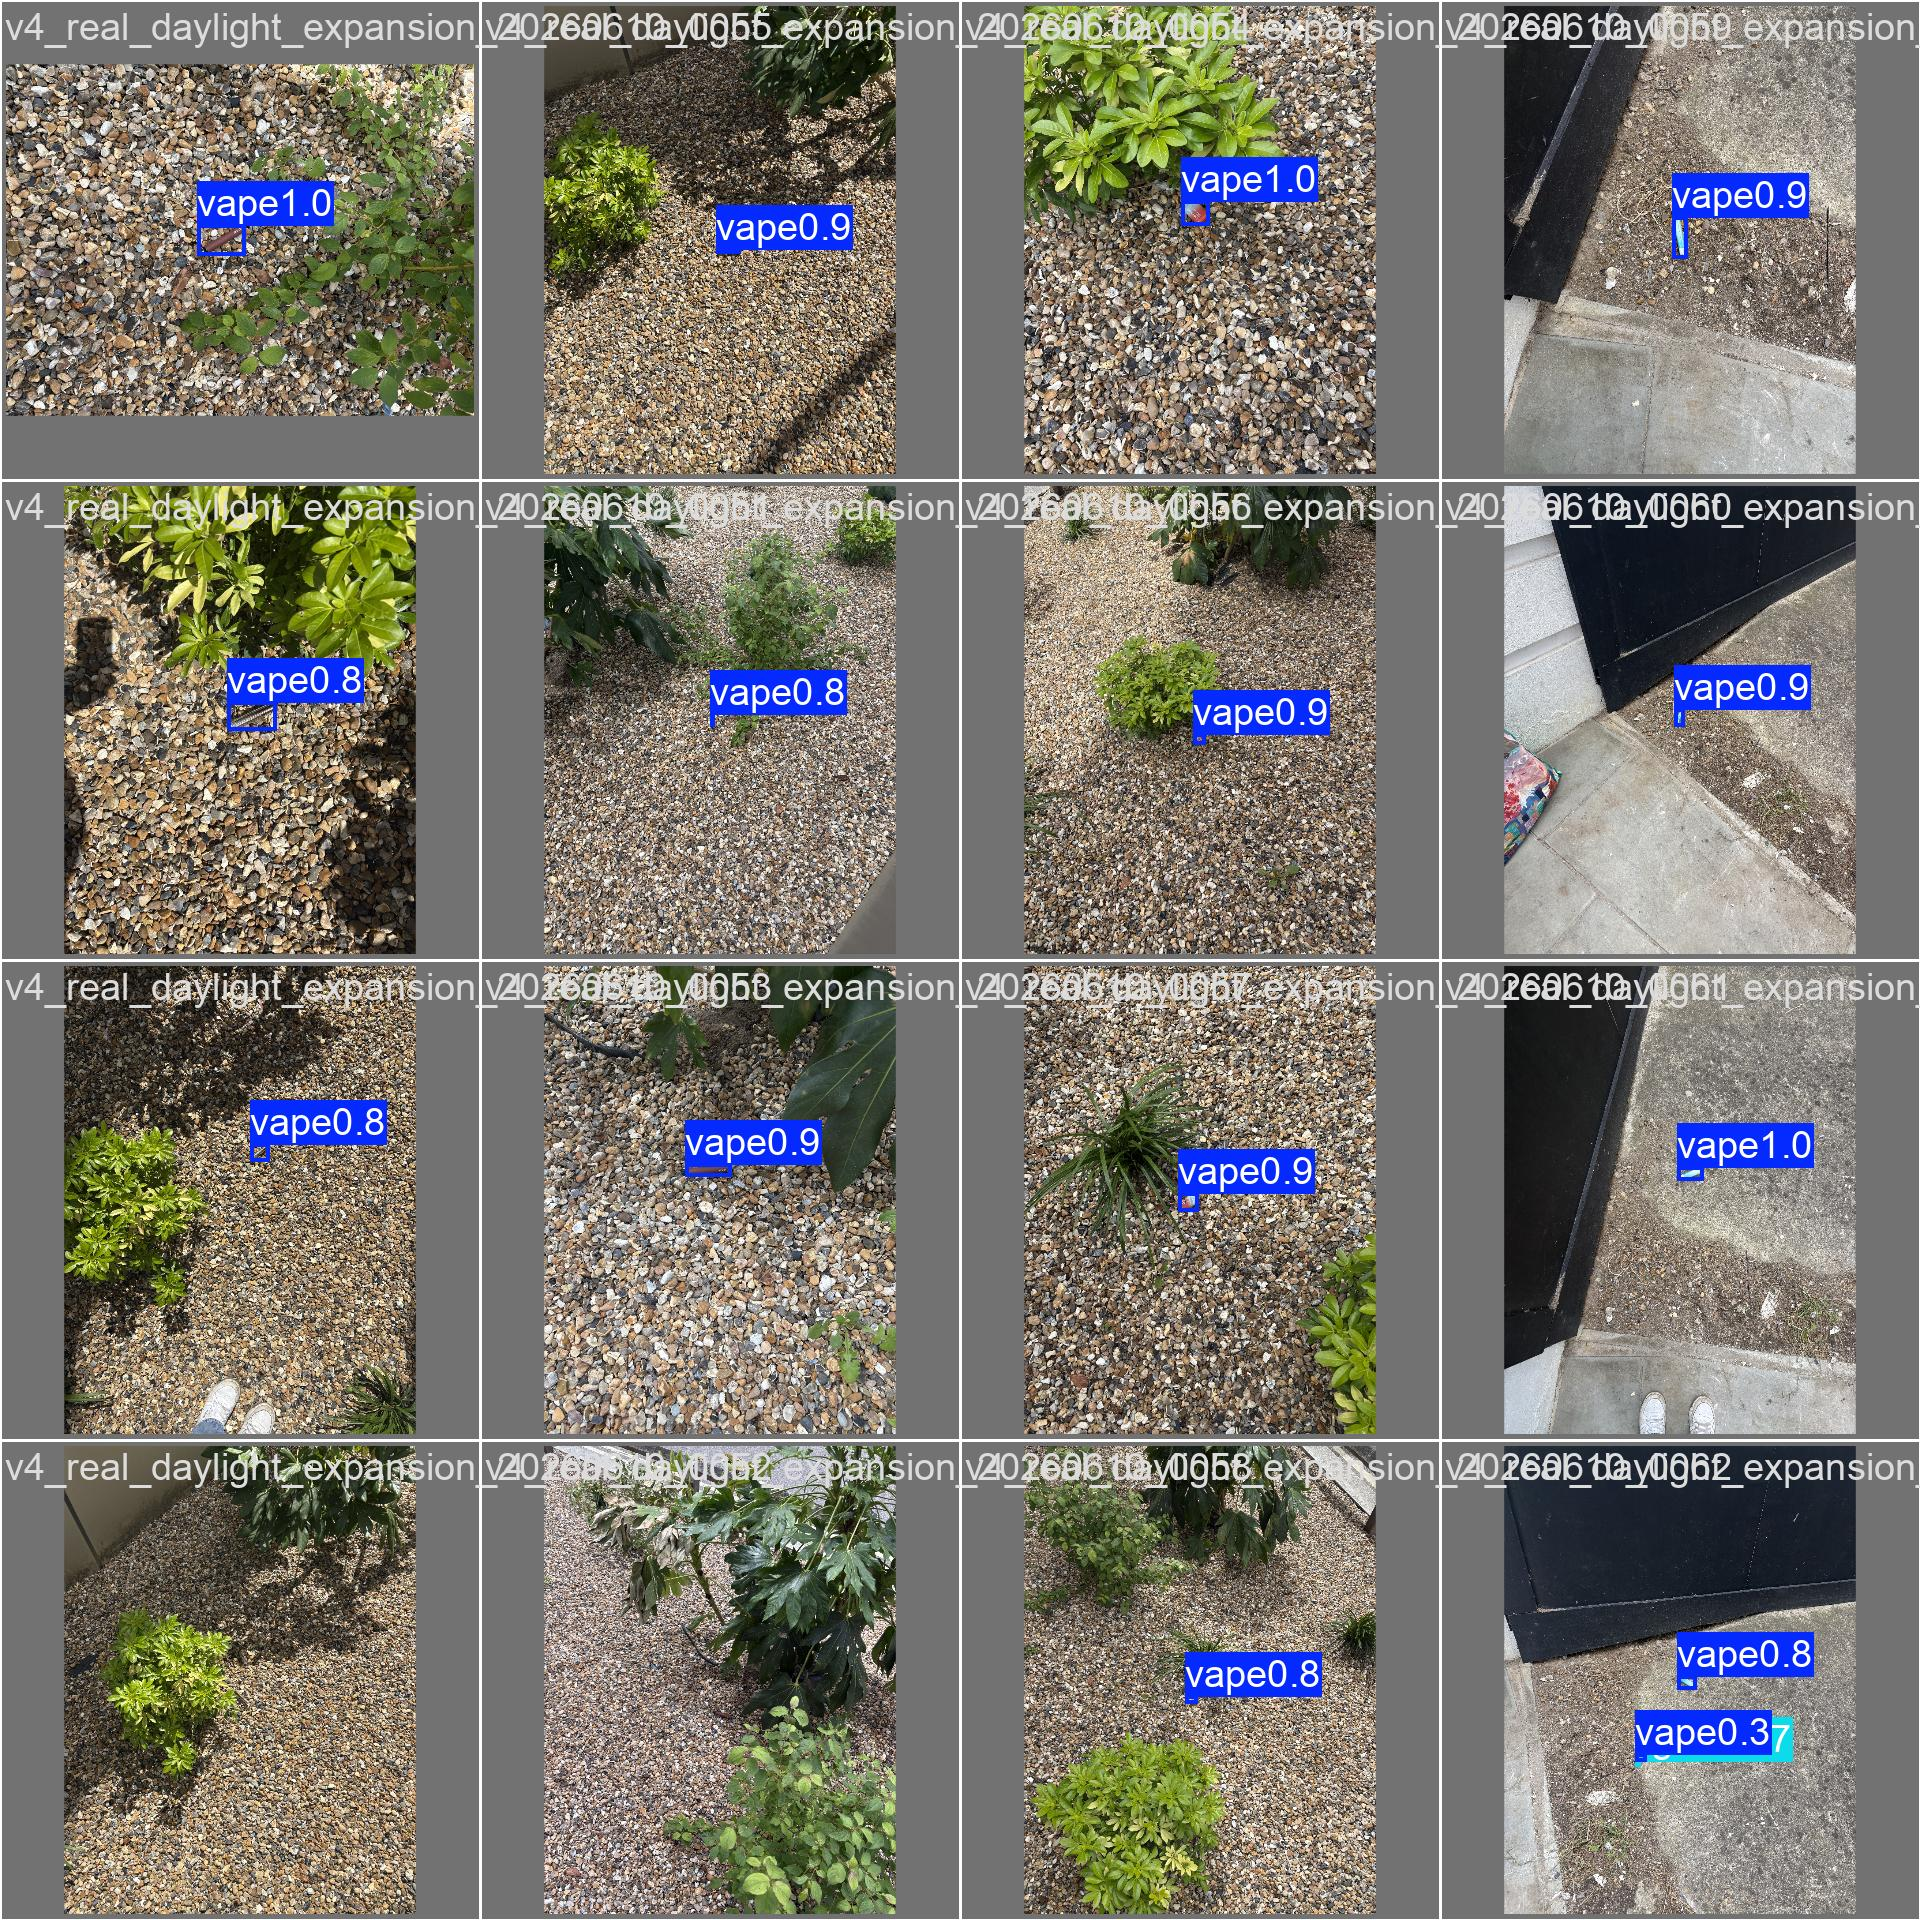
\includegraphics[width=0.95\linewidth]{final_test_val_batch0_pred.jpg}
    \caption{Final sealed-test prediction preview, batch 0. Predicted vape and lighter detections are shown on held-out real test images.}
    \label{fig:appendix_final_test_batch0_pred}
\end{figure}

\begin{figure}[H]
    \centering
    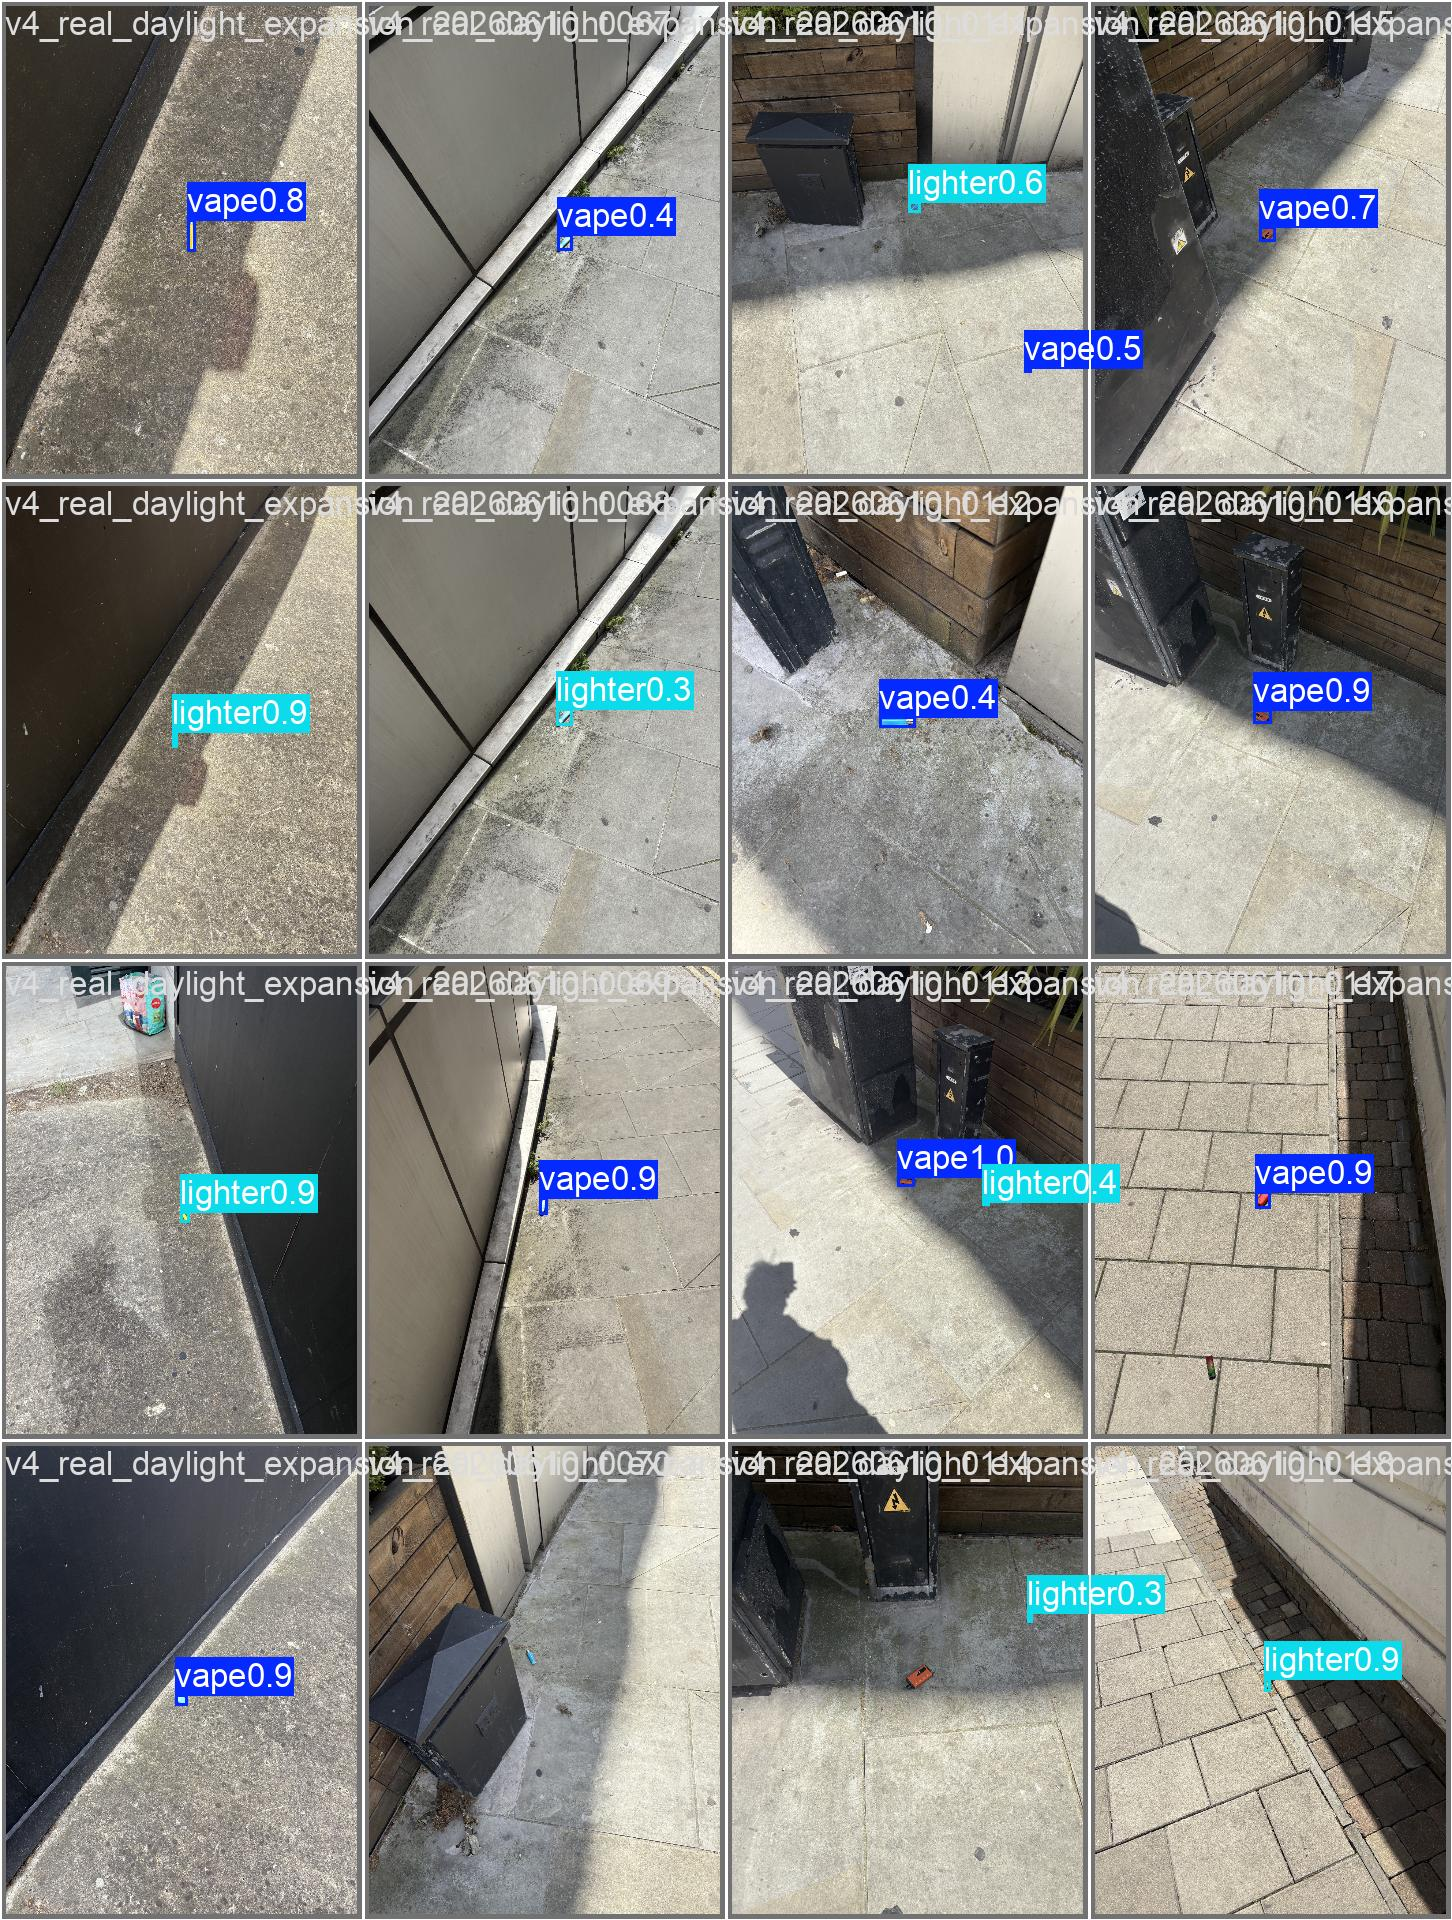
\includegraphics[width=0.95\linewidth]{final_test_val_batch1_pred.jpg}
    \caption{Final sealed-test prediction preview, batch 1. This preview provides qualitative evidence of detector behaviour across additional held-out test examples.}
    \label{fig:appendix_final_test_batch1_pred}
\end{figure}

\begin{figure}[H]
    \centering
    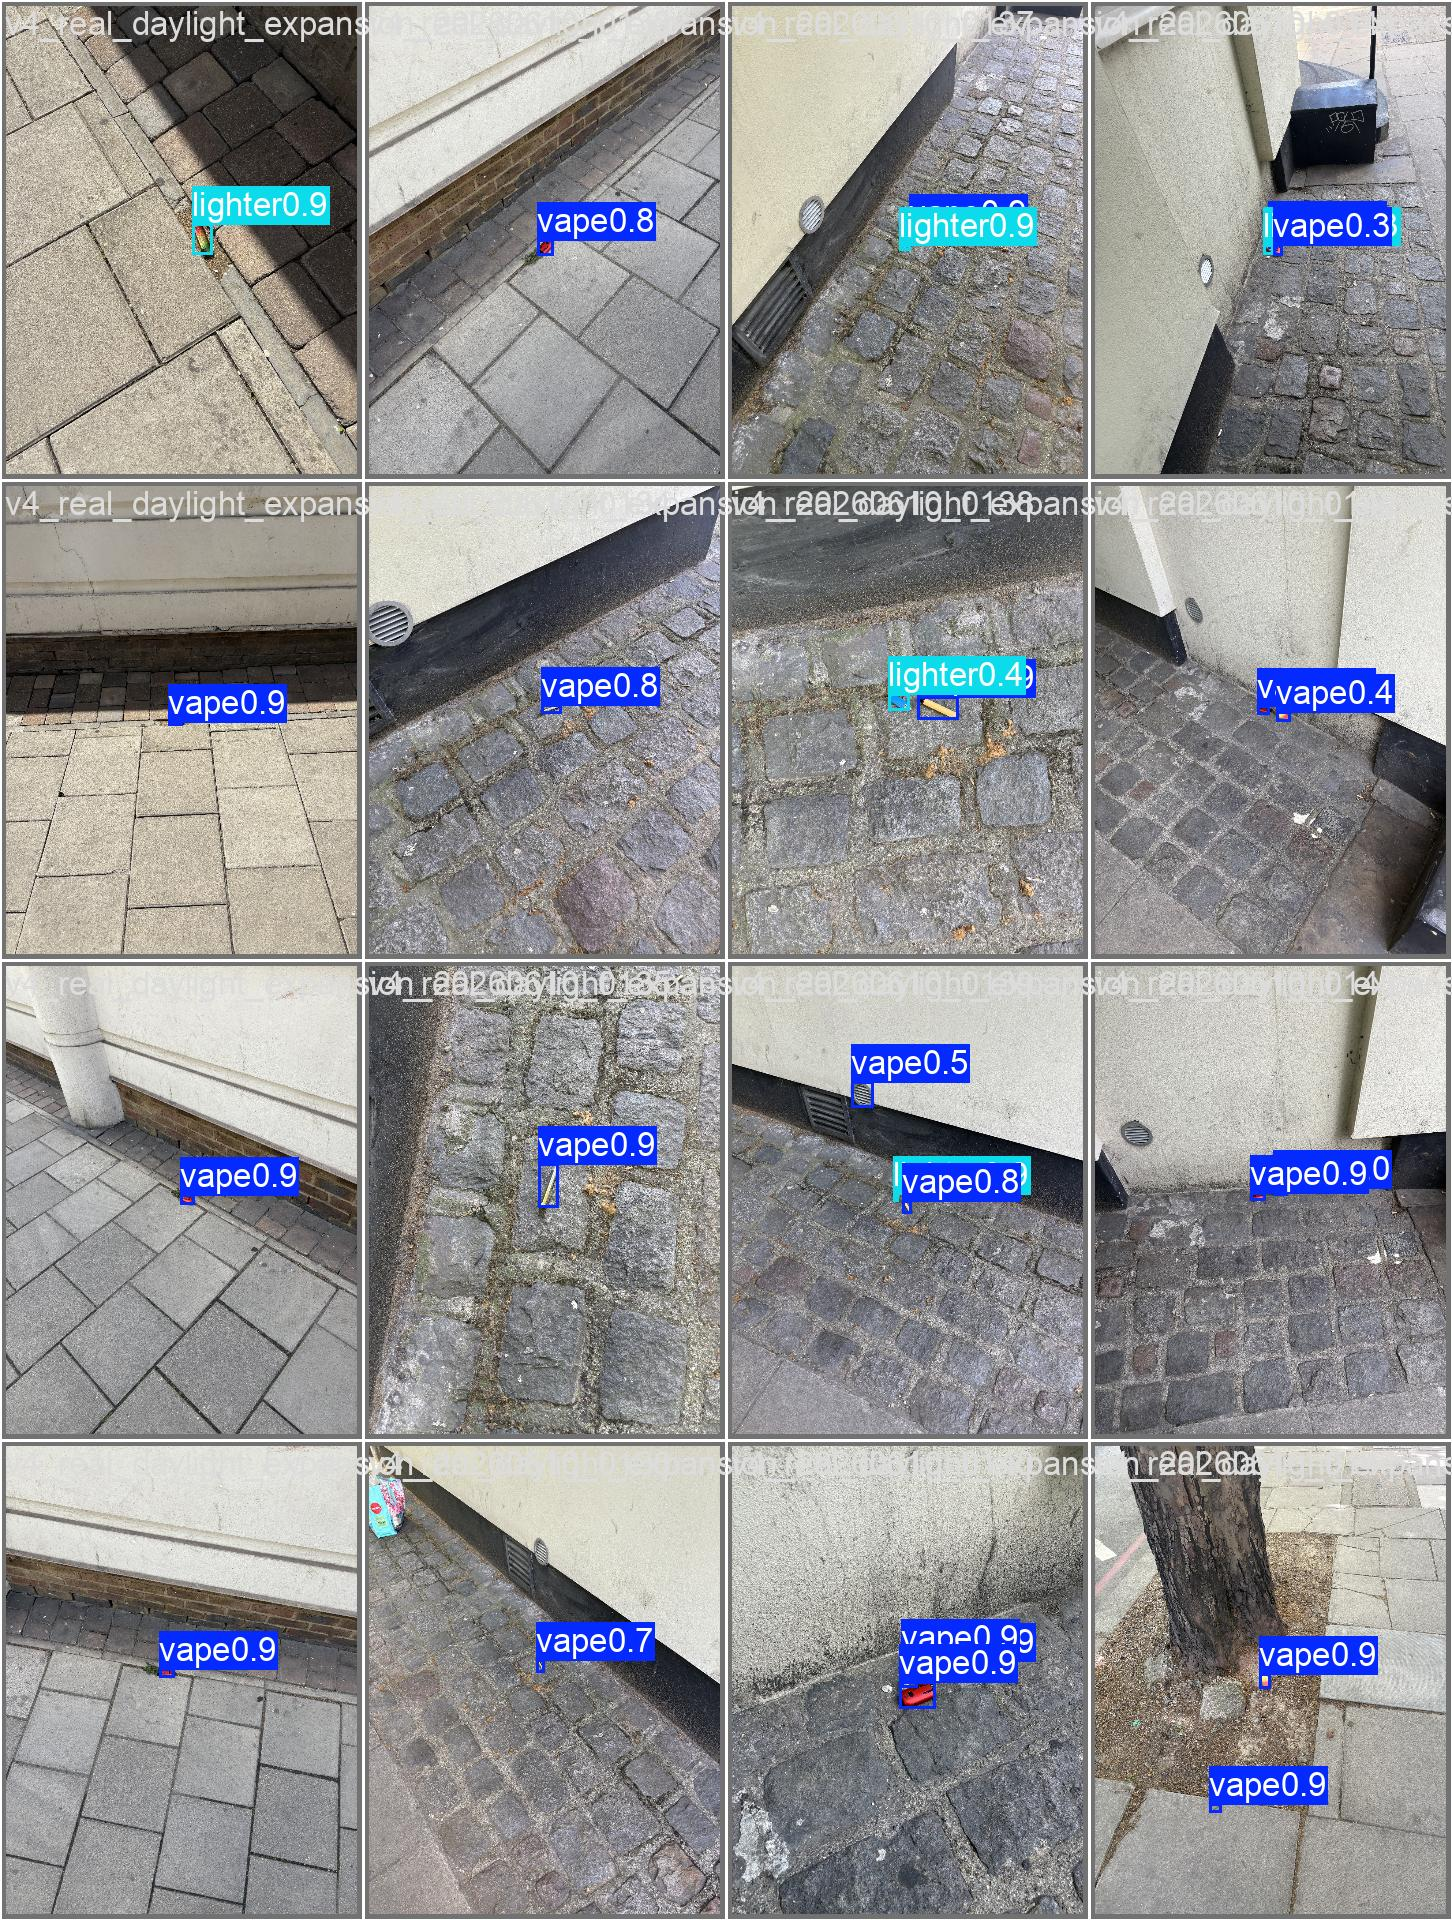
\includegraphics[width=0.95\linewidth]{final_test_val_batch2_pred.jpg}
    \caption{Final sealed-test prediction preview, batch 2. The preview helps contextualise the final AP metrics by showing the detector's bounding-box outputs on unseen real images.}
    \label{fig:appendix_final_test_batch2_pred}
\end{figure}

\section{UAVape Model Repository}
\label{app:uavape_model_repository}
\textit{TODO: Insert final GitHub repository link for the UAVape model benchmark and result artifacts.}

This repository should contain the model-training notebooks or scripts, configuration files, validation benchmark outputs, SAHI/tiling evidence, data-source ablation results, final sealed-test output and README instructions for reproducing the reported model results.

\section{Dataset Construction Engine (DCE) Repository}
\label{app:dce_repository}
\textit{TODO: Insert final GitHub repository link for the Dataset Construction Engine.}

This repository should contain the DCE source code, setup instructions, screenshots or interface captures, and README documentation explaining the intake, curation, SAM2-assisted annotation, metadata, audit and COCO/YOLO export workflow.

\subsubsection{System Architecture and Implemented Workflow}

The implemented DCE used a React/FastAPI and Python data-processing architecture. The frontend handled review, metadata, annotation and audit/export interactions. The backend managed dataset state, file operations and service orchestration. Python services handled collection, ingest, duplicate handling, SAM-assisted annotation, COCO audit and YOLO export.

\begin{figure}[H]
    \centering
    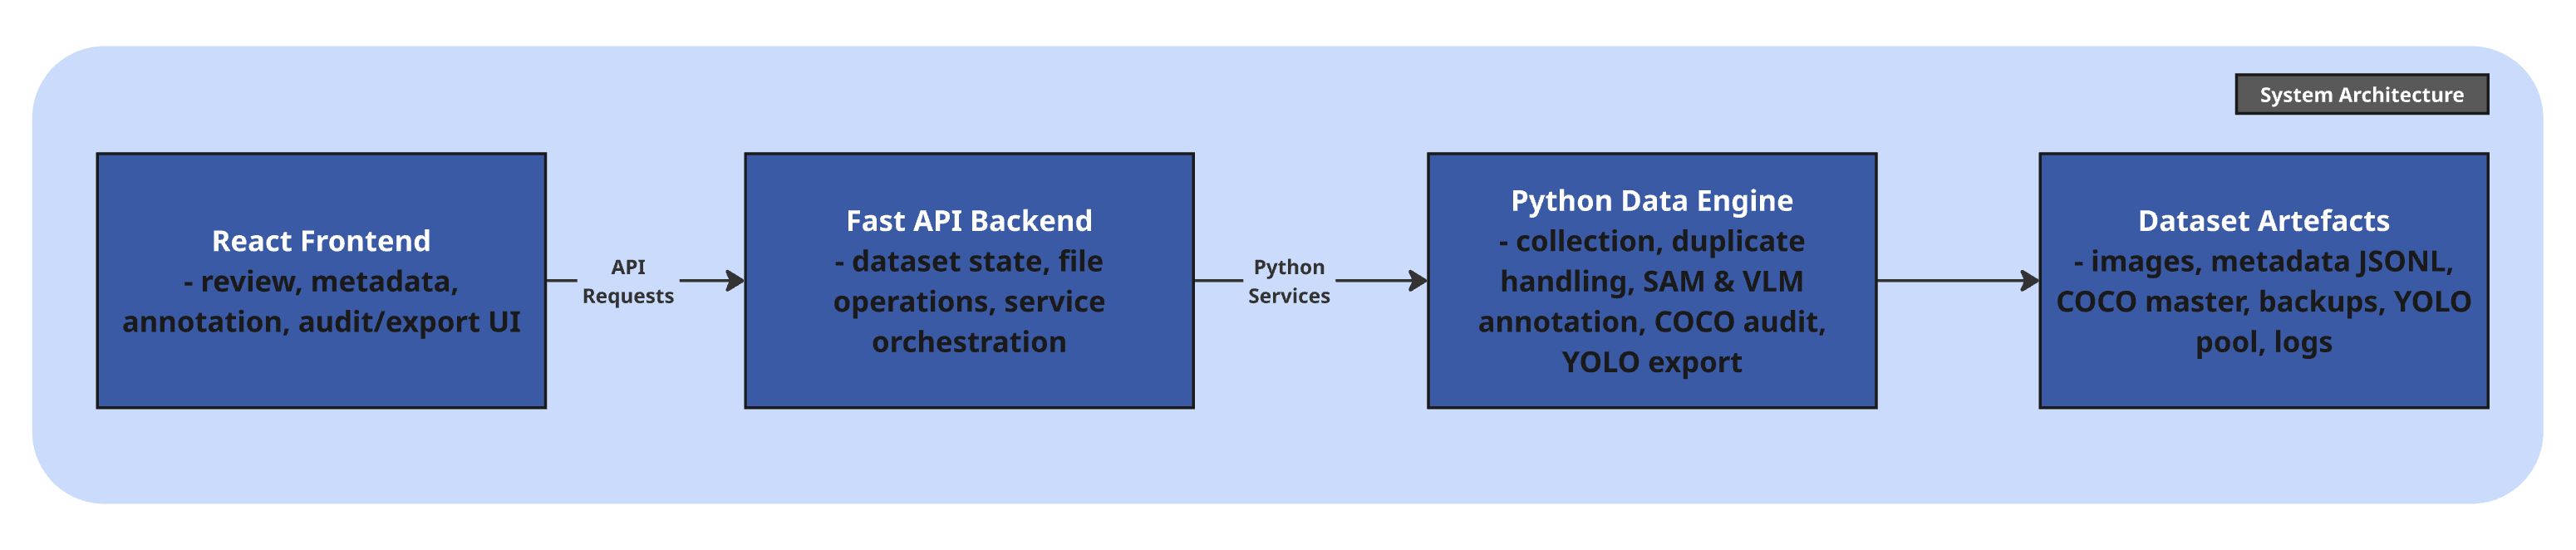
\includegraphics[width=1\linewidth]{sysarch.png}
    \caption{DCE System Architecture}
    \label{fig:appendix_dce_system_architecture}
\end{figure}

\section{UAVape Cleanup Planner UI Repository}
\label{app:cleanup_planner_repository}
\textit{TODO: Insert final GitHub repository link for the UAVape Cleanup Planner prototype.}

This repository should contain the clickable HTML prototype, high-resolution interface captures, survey wrapper and any supporting assets used during the stakeholder walkthrough. The prototype evidence is separated from the DCE and model repositories because it represents the cleaner-facing workflow contribution rather than the dataset or detector implementation.

The prototype was evaluated against the current questions:
\begin{table}[H]
\centering
\small
\begin{tabularx}{\textwidth}{p{0.10\textwidth} X p{0.25\textwidth}}
\toprule
\textbf{Question} & \textbf{Survey item} & \textbf{Response type} \\
\midrule
Q1 & The evidence crop made it easier to understand what item needed to be collected. & Five-point Likert \\
Q2 & The map point gave enough location context to support field collection. & Five-point Likert \\
Q3 & Showing the model confidence score helped me judge whether the detection should be trusted or reviewed. & Five-point Likert \\
Q4 & Labelling disposable vapes as hazardous micro-WEEE made the task feel different from ordinary litter collection. & Five-point Likert \\
Q5 & The supervisor dashboard made it clear which detections required attention first. & Five-point Likert \\
Q6 & The task queue provided enough information to assign cleanup work to a team or individual. & Five-point Likert \\
Q7 & The cleaner phone task view was simple enough to use during outdoor fieldwork. & Five-point Likert \\
Q8 & The status options, collected, not found and needs review, were appropriate for recording field outcomes. & Five-point Likert \\
Q9 & Overall, the workflow would improve task clarity compared with current manual or route-based cleanup methods. & Yes/no/unsure \\
Q10 & What is the main practical barrier that would prevent this workflow from being used during real cleanup work? & Open text \\
\bottomrule
\end{tabularx}
\caption{Cleaner workflow stakeholder survey instrument.}
\label{tab:appendix_cleaner_method_survey}
\end{table}

\section{Project Management}
\label{app:project_management}
\begin{figure}[H]
    \centering
    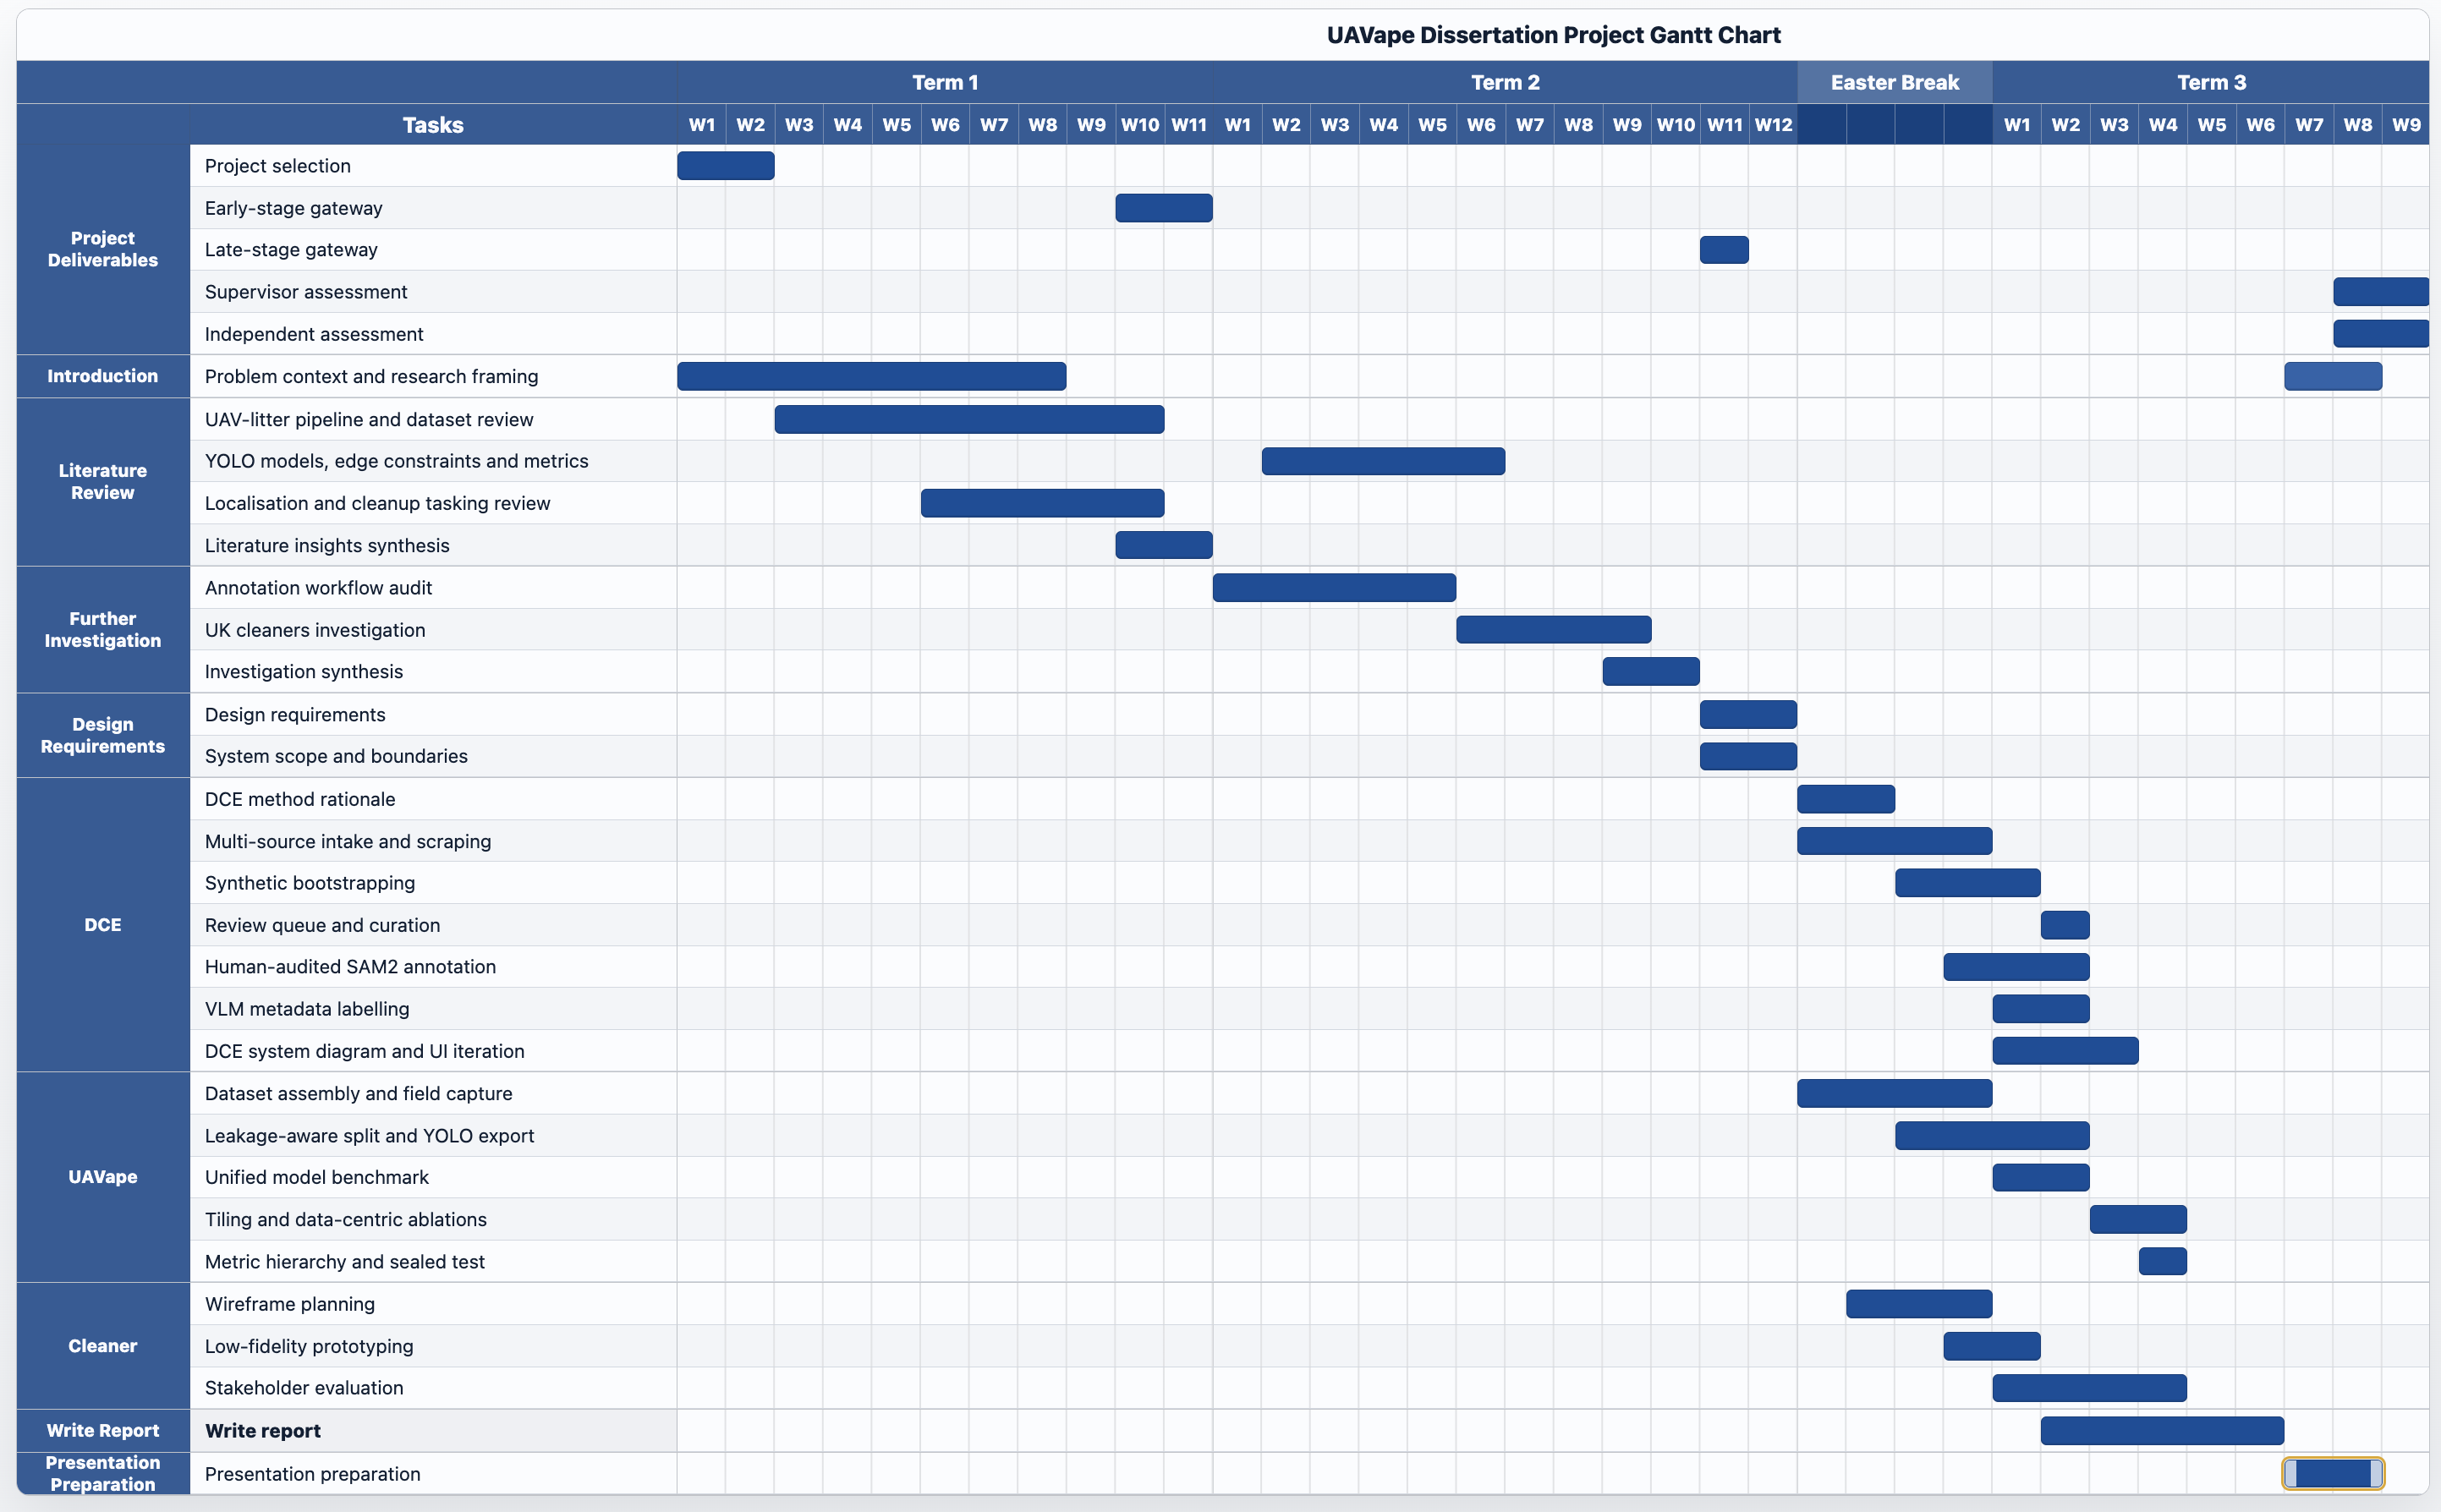
\includegraphics[width=1\linewidth]{Gantt.png}
    \caption{Project Gantt Chart detailing timeline and milestones.}
    \label{fig:gantt_chart}
\end{figure}
\textit{TODO: Insert Excel/OneDrive link for the full project logbook.}

The project objectives and scope underwent iterative refinement in response to emergent findings. The full project logbook should document the major timeline changes, scope adjustments, implementation milestones and project-management decisions that supported the final dissertation structure.

\section{Extended Reflection: Note From Author}
\label{app:extended_reflection}
\textit{Note From Author:}

This project was a massive interdisciplinary effort. At its core, it brought together data science, data engineering, machine learning, software engineering, and finally human-centred design engineering. The UAVape dataset, the Dataset Construction Engine, and the machine learning model required one type of thinking: technical, systematic, and deeply detailed. The cleaner workflow concept required another type of thinking: user-centred, practical, and focused on whether the technology could actually mean anything to the people on the ground.

This naturally came about from wanting to build an end-to-end solution. If you actually try to solve a real problem properly, you very quickly realise that the solution cannot sit inside one discipline. It needs data, it needs software, it needs machine learning, it needs design, and it needs people. That is something I had already begun to appreciate through previous projects in the MEng Design Engineering course, but UAVape made it feel much more real.

Looking back, I realised that I could have taken a much simpler route. I could have just scraped some vape images, annotated them, trained a model, and ended the project there. I could have used one type of data, or built a smaller dataset, or avoided the complexity of synthetic data, staged data, scraped data, real-world data, auxiliary confuser classes, metadata, and the whole Dataset Construction Engine. But I chose not to do that because I wanted to genuinely put my best foot forward. I wanted to create the most complete approach I could, not just something that technically worked.

The more I worked on the dataset, the more I realised that image detection for vapes only seems simple on the surface. At first, it sounds like a basic machine learning task: collect images of vapes, label them, and train a detector. But when you get into the details, it becomes much more complex. Vapes come in different shapes, colours, sizes, brands, conditions, and contexts. They look like pens, markers, cables, wrappers, batteries, and other bits of litter. They can be close-up, far away, partially hidden, blurred, or tiny in the frame. Suddenly, the problem is not just ``detect a vape.'' It becomes a whole question of what kind of data is good enough, what kind of annotation is trustworthy enough, and what kind of system is needed to make that process repeatable.

That was one of the most intellectually stimulating parts of the project for me. I found myself in territory that felt genuinely unexplored. I was reading deeper and deeper into machine learning, dataset construction, object detection, annotation formats, failure modes, and UAV litter research. And the more I read, the more I understood why the Dataset Construction Engine was justified. It was not just a tool I built because I needed a dataset. It became a way of exploring an underdeveloped problem: how do you actually create reliable, detection-ready data for a new and specific object class like disposable vape litter?

I appreciate that the cleaner workflow side of the project was something that could have easily been scoped out. The dataset construction engine alone became a huge project. It had enough technical depth, enough implementation work, and enough validation to stand on its own. But I did not want the project to stop at the point where a model detects an object and produces a number. After four years of Design Engineering, I have learned that user-centered work is not just an extra layer you add at the end. It is the pragmatic way to make systems actually matter.

That is why I kept the cleaner workflow in the project. It was my attempt to connect the technical side of the work with the real human side of litter cleanup. The world of machine learning, UAV detection, datasets, and model metrics is so far removed from the world of municipal workers, cleaners, volunteers, and people physically removing waste from public spaces. Those two worlds rarely touch. The people building the technology may never pick litter. The people picking litter may never have access to the technology. Someone has to connect them.

That was what I tried to do with UAVape. I wanted to show that it is not enough for technology to simply explore new territory or achieve better metrics. It also has a responsibility to become useful. A detection should not just stay as a bounding box. It should become evidence, a map point, a task, a status, and eventually something that helps a real person do their work better. That was the point of the workflow concept: to take something highly technical and translate it into something operational, understandable, and human.

In that sense, UAVape became a full expression of what I think Design Engineering has taught me. It taught me that building a solution properly means moving between levels: from code to data, from data to models, from models to systems, and from systems to people. It taught me that technical ambition matters, but so does humility about how technology is actually used. It taught me that the most interesting problems are often the ones that look simple at first, but become deeper the more seriously you take them.

This project was difficult, but I loved that difficulty. I loved the intellectual depth of it, the fact that every layer opened up another layer, and the fact that it forced me to use almost everything I had learned across the degree. It was not just a machine learning project, and it was not just a design project. It was a real design engineering project: technical, messy, interdisciplinary, human, and aimed at making something that could actually connect to the world, but obviously within the bounds of it being testable research and the time constraints of the project.

\section{AI Declaration}
All concepts, research, academic arguments and system designs are entirely the author's work. Generative AI tools, specifically ChatGPT and Gemini were used to assist the following:

For software engineering, AI helped generate and debug code. On the Python backend, it helped write standard boilerplate code, set up libraries, and read error logs to fix bugs. On the React frontend, it helped build interface components and update the code when the author--for example--changed the layout, like moving from drop-down lists to modal windows or tables.

When writing the report, AI tools were used to check diction, fix grammar, and improve conciseness. Most importantly, as the document was completed in Overleaf, AI assisted in troubleshooting LaTeX code, managing document packages, and aligning data tables and TikZ graphics.

It is important to reiterate that every single idea was entirely the author's. The content throughout the report is extremely precise and detailed and fundamentally derived from real work, therefore ideas and analysis could only be done by the author.

Ultimately, every final design choice, qualitative evaluation, and engineering decision remains the author's independent work.

